\chapter{Results of the SM measurement}
\label{chap:results}
This chapter shows the results of the likelihood fit introduced in section~\ref{sec:likelihood}.
Finally the signal strength $\mu$ is extracted and the observed significance is estimated.

\section{Post fit plots}
%\noindent\textbf{\sf{$m^{tag}_{jj}$ distributions at CRs after fitting}}\\
\subsection{ $m^{tag}_{jj}$ distributions at CRs after fitting }
The distributions used in the final fitting are shown to check if it performed well.
The $m^{tag}_{jj}$ distributions in each CRs after fitting are shown in figure~\ref{fig:postCR} and \ref{fig:postCRTop}.
The MC predictions match to the data well in all CRs after fitting. 

%Control region
\begin{figure}[H]
    \centering
    %0lep
    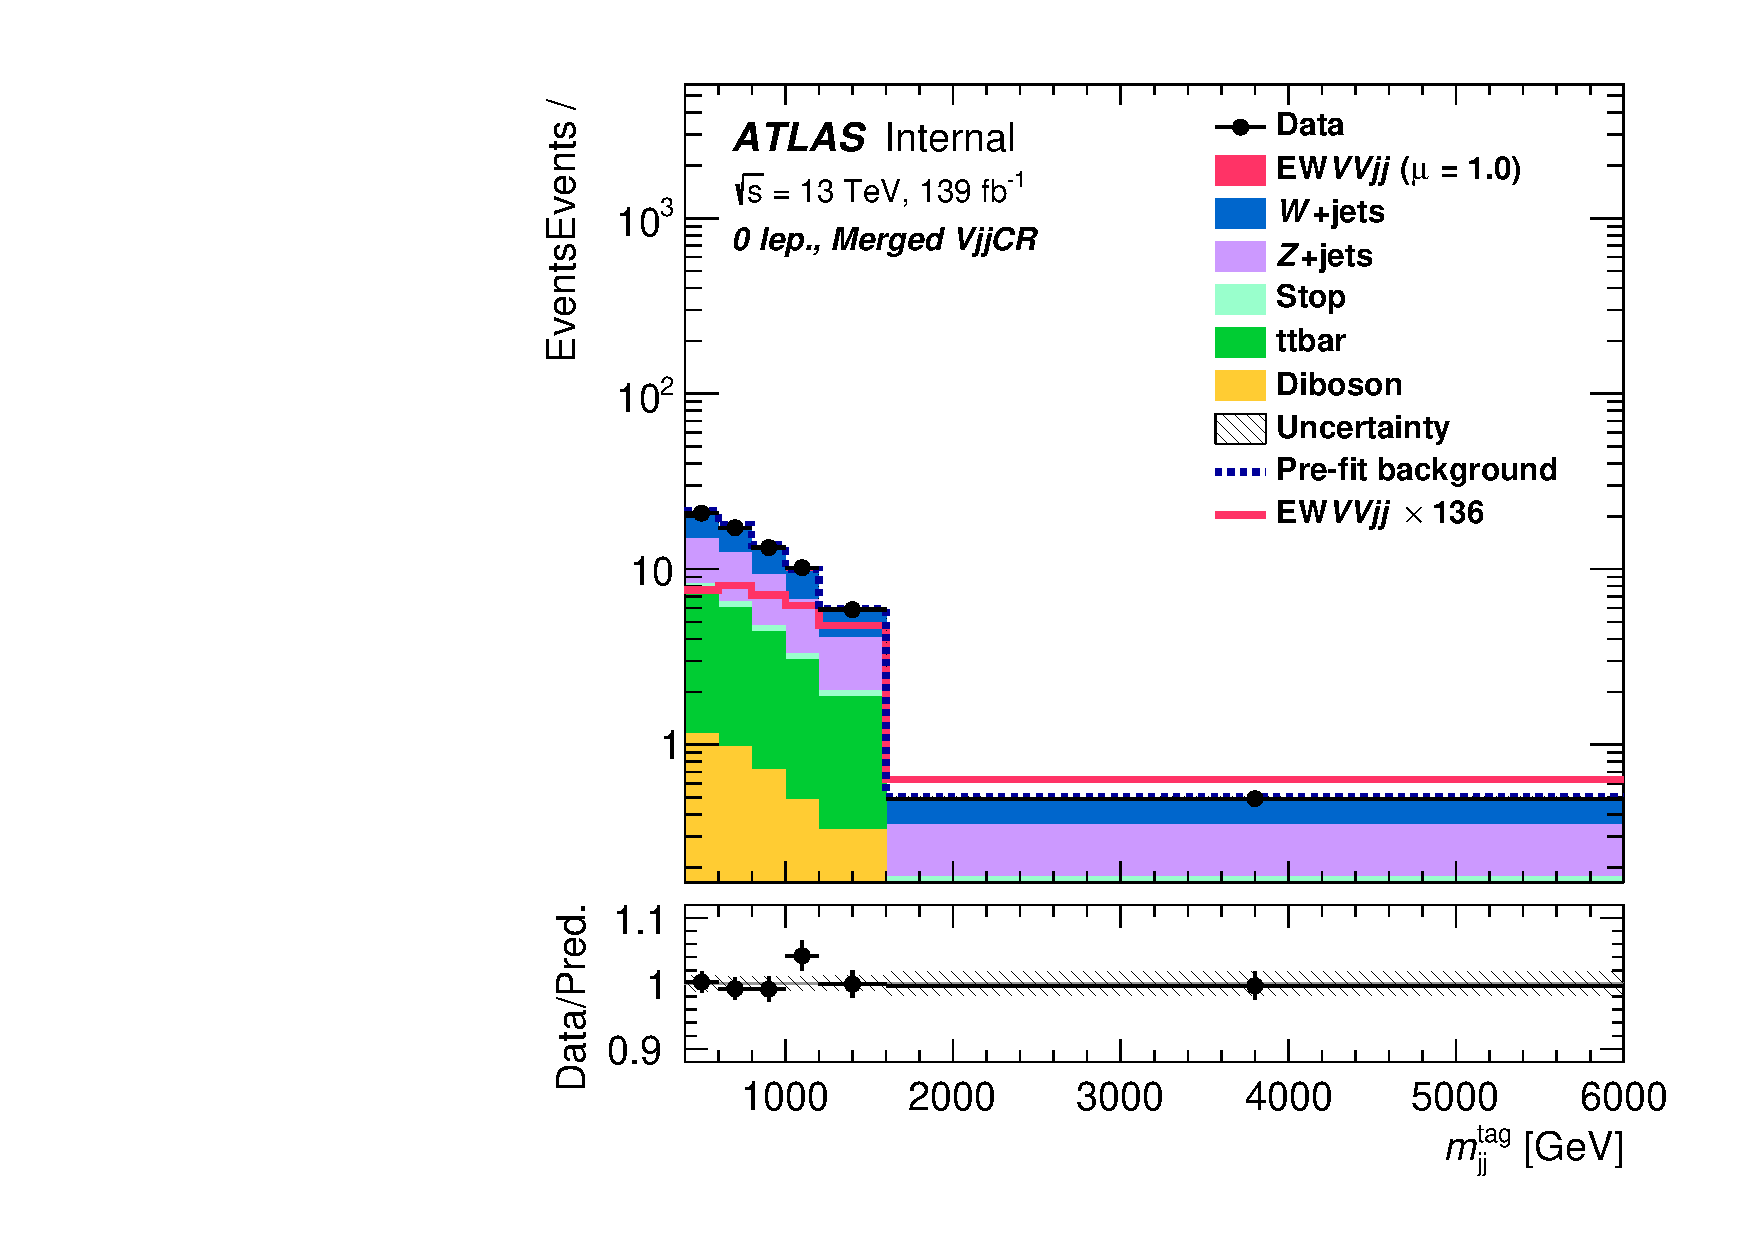
\includegraphics[width=0.45\textwidth]{figures/PostFit/Region_distMTagJets_DCRVjetMer_BMin0_J0_incJet1_L0_T0_incFat1_Y6051_incTag1_Fat1_GlobalFit_unconditionnal_mu1log}
    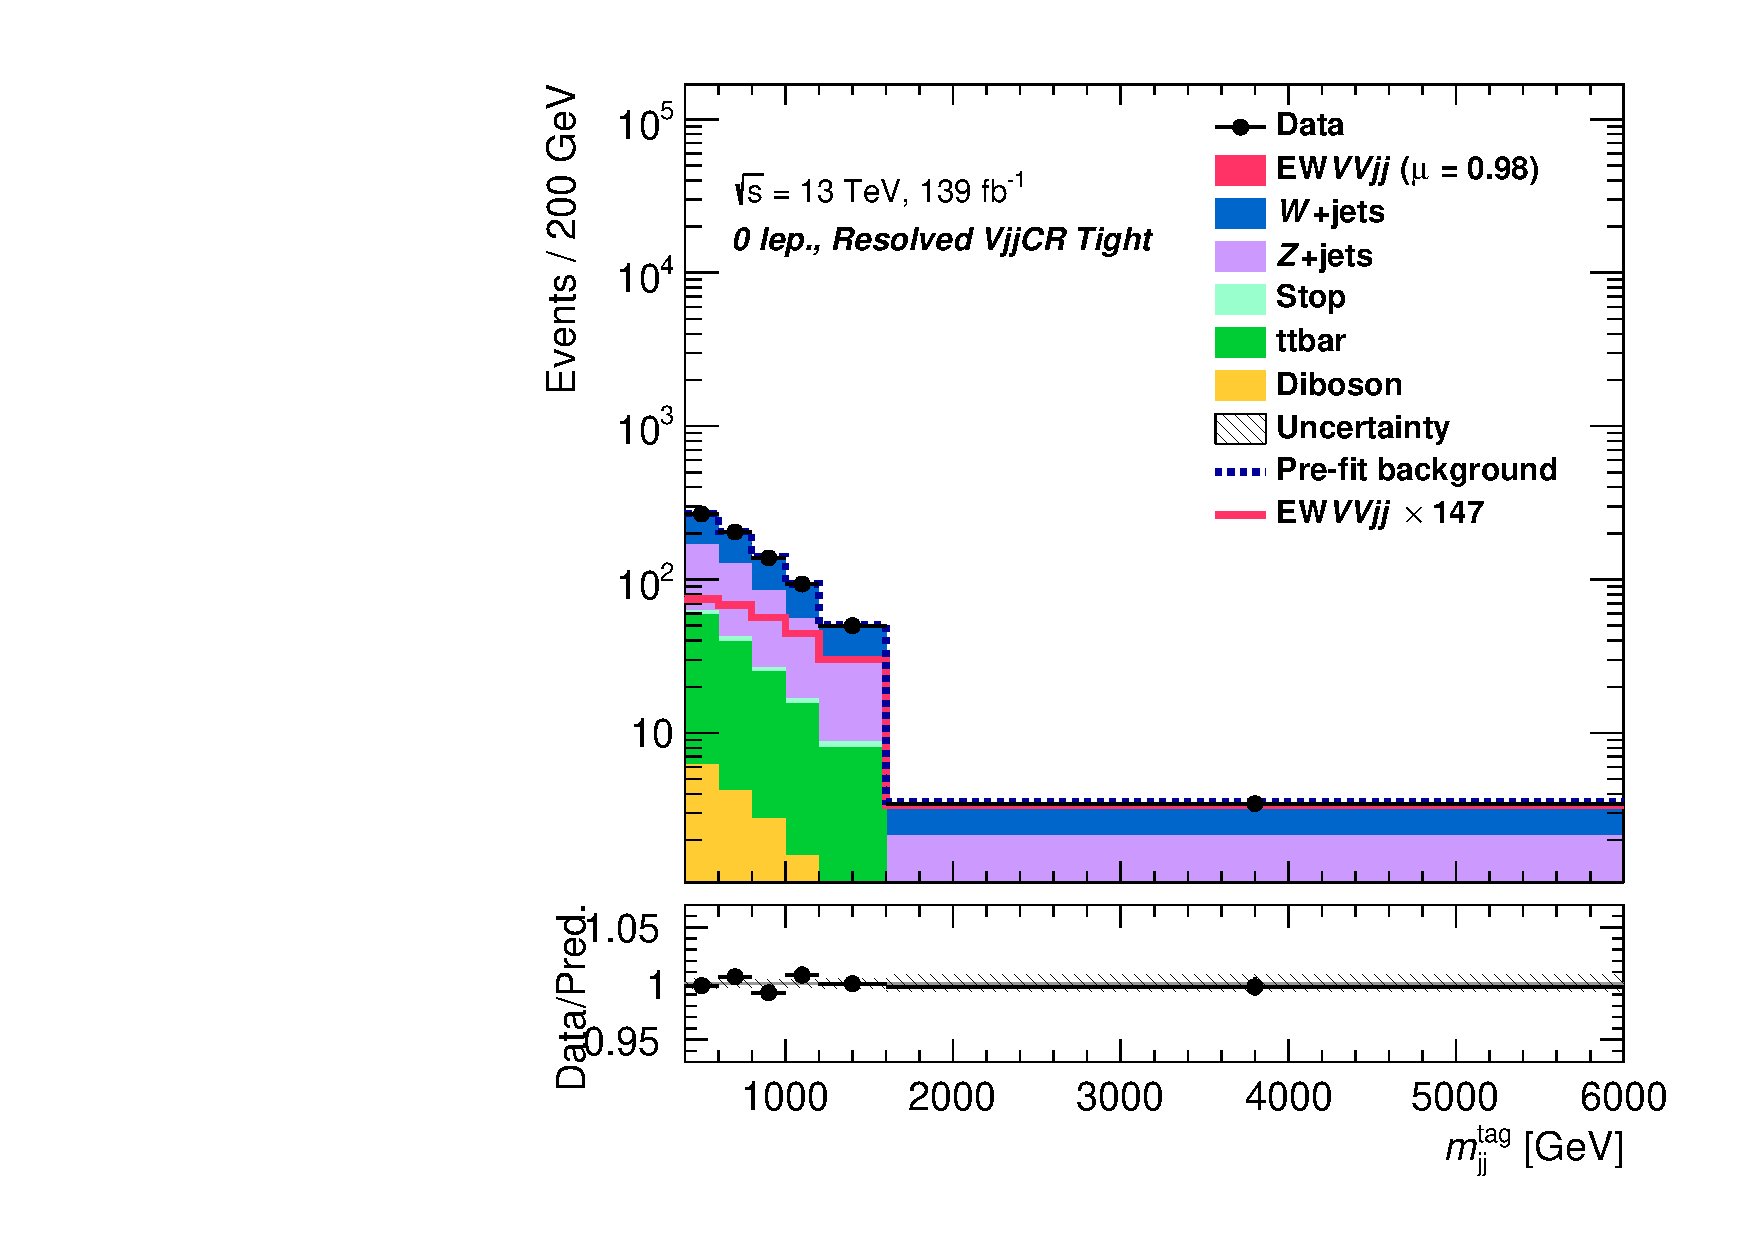
\includegraphics[width=0.45\textwidth]{figures/PostFit/Region_distMTagJets_DCRVjetFid_BMin0_T0_Y6051_incTag1_J2_L0_incJet1_GlobalFit_unconditionnal_mu1log}
    \\
    %1lep
    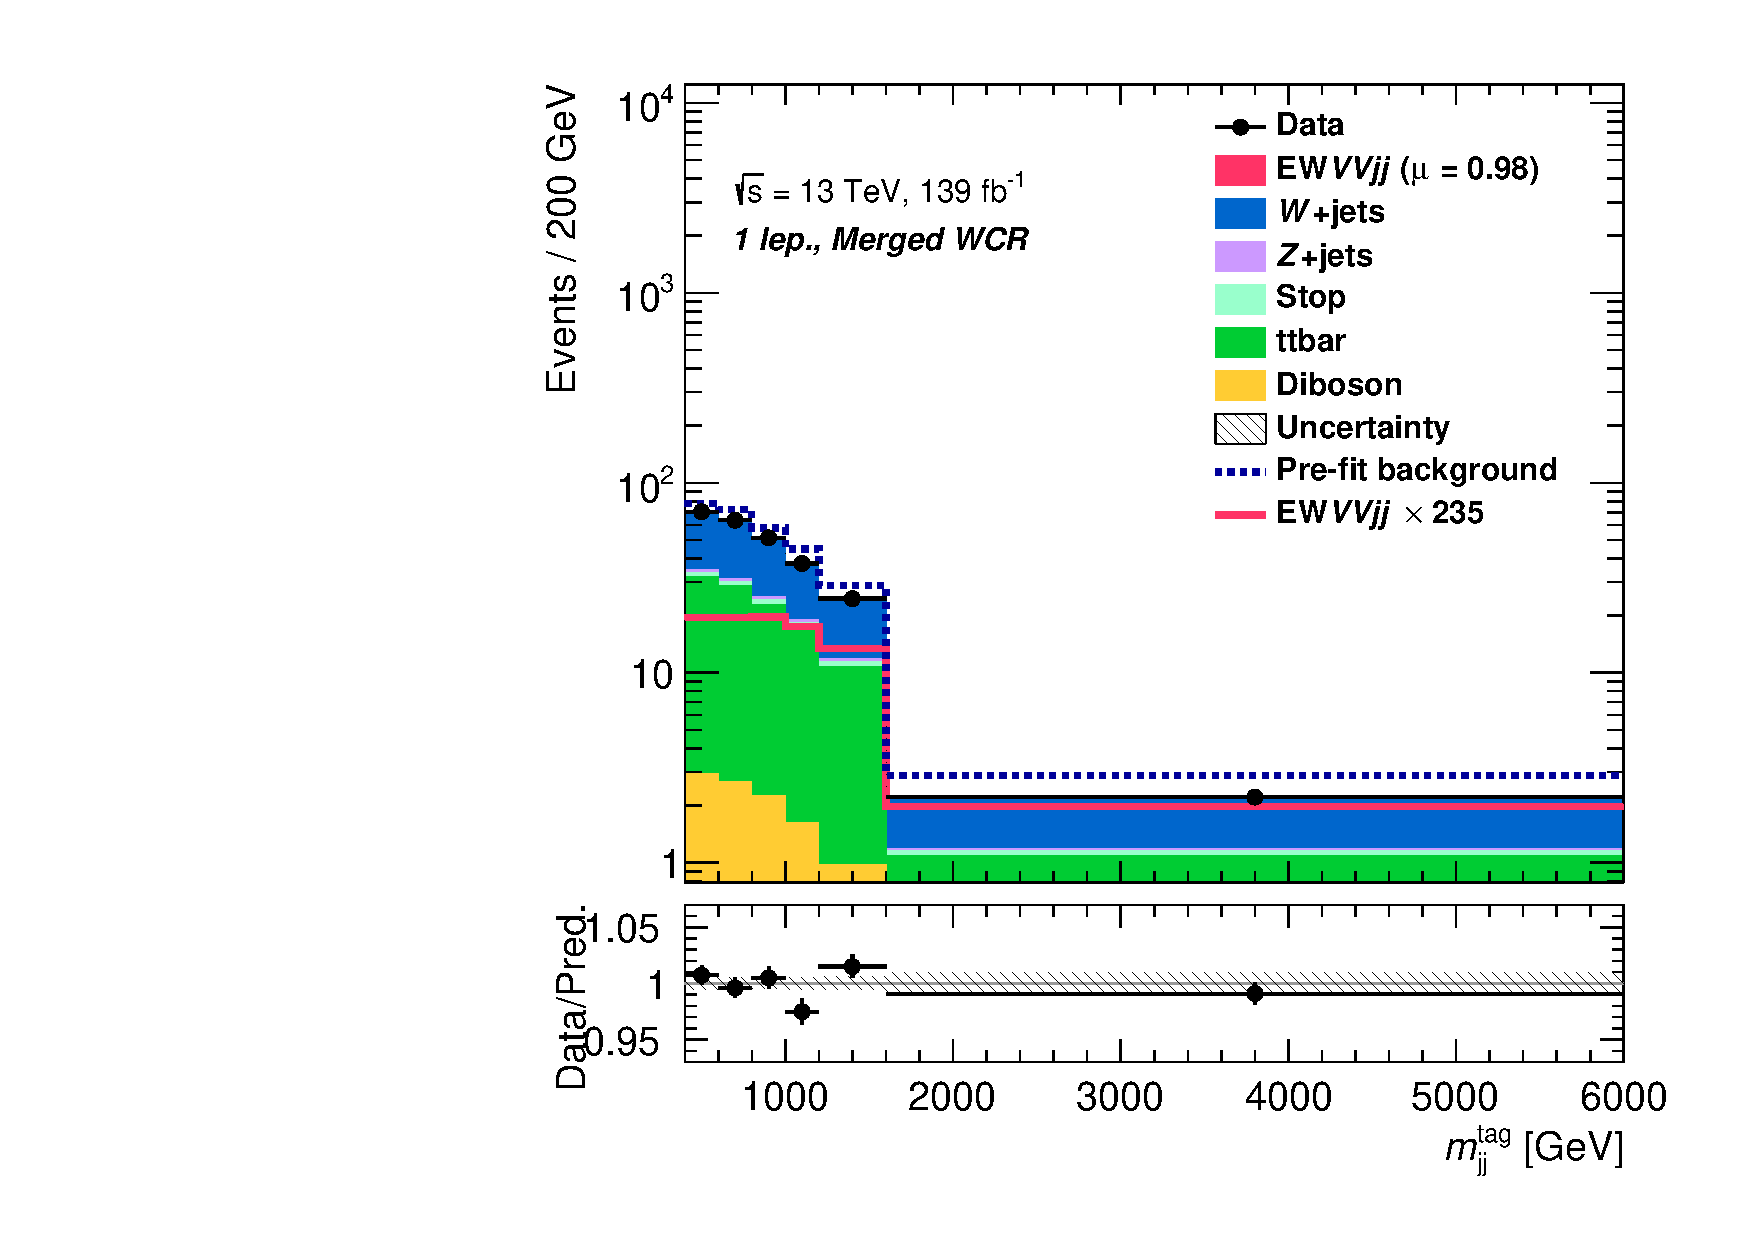
\includegraphics[width=0.45\textwidth]{figures/PostFit/Region_disttagMjj_DCRVjetMerged_BMin0_J0_incJet1_L1_T0_incFat1_Y6051_incTag1_Fat1_GlobalFit_unconditionnal_mu1log}
    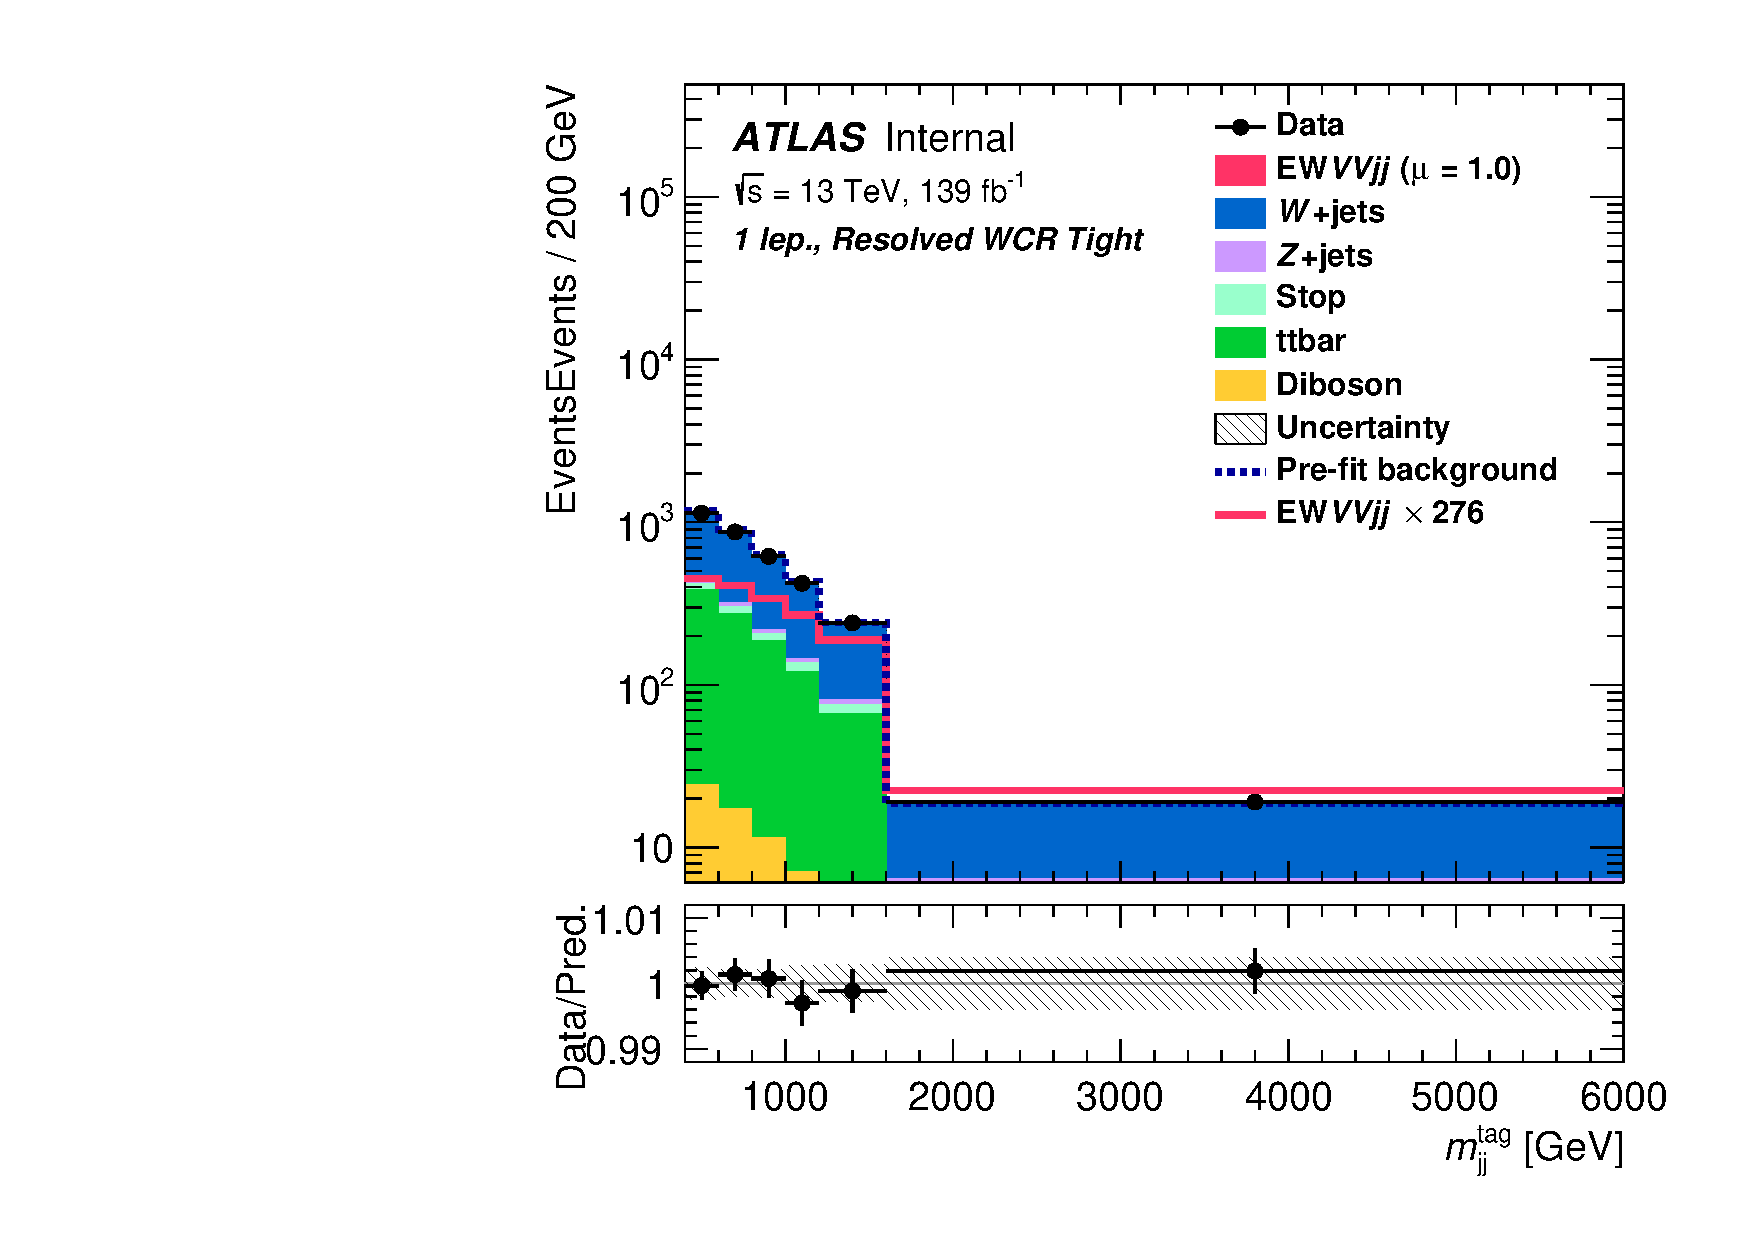
\includegraphics[width=0.45\textwidth]{figures/PostFit/Region_disttagMjj_DCRVjetTight_BMin0_T0_Y6051_incTag1_J2_L1_incJet1_GlobalFit_unconditionnal_mu1log}
    \\
    %2lep
     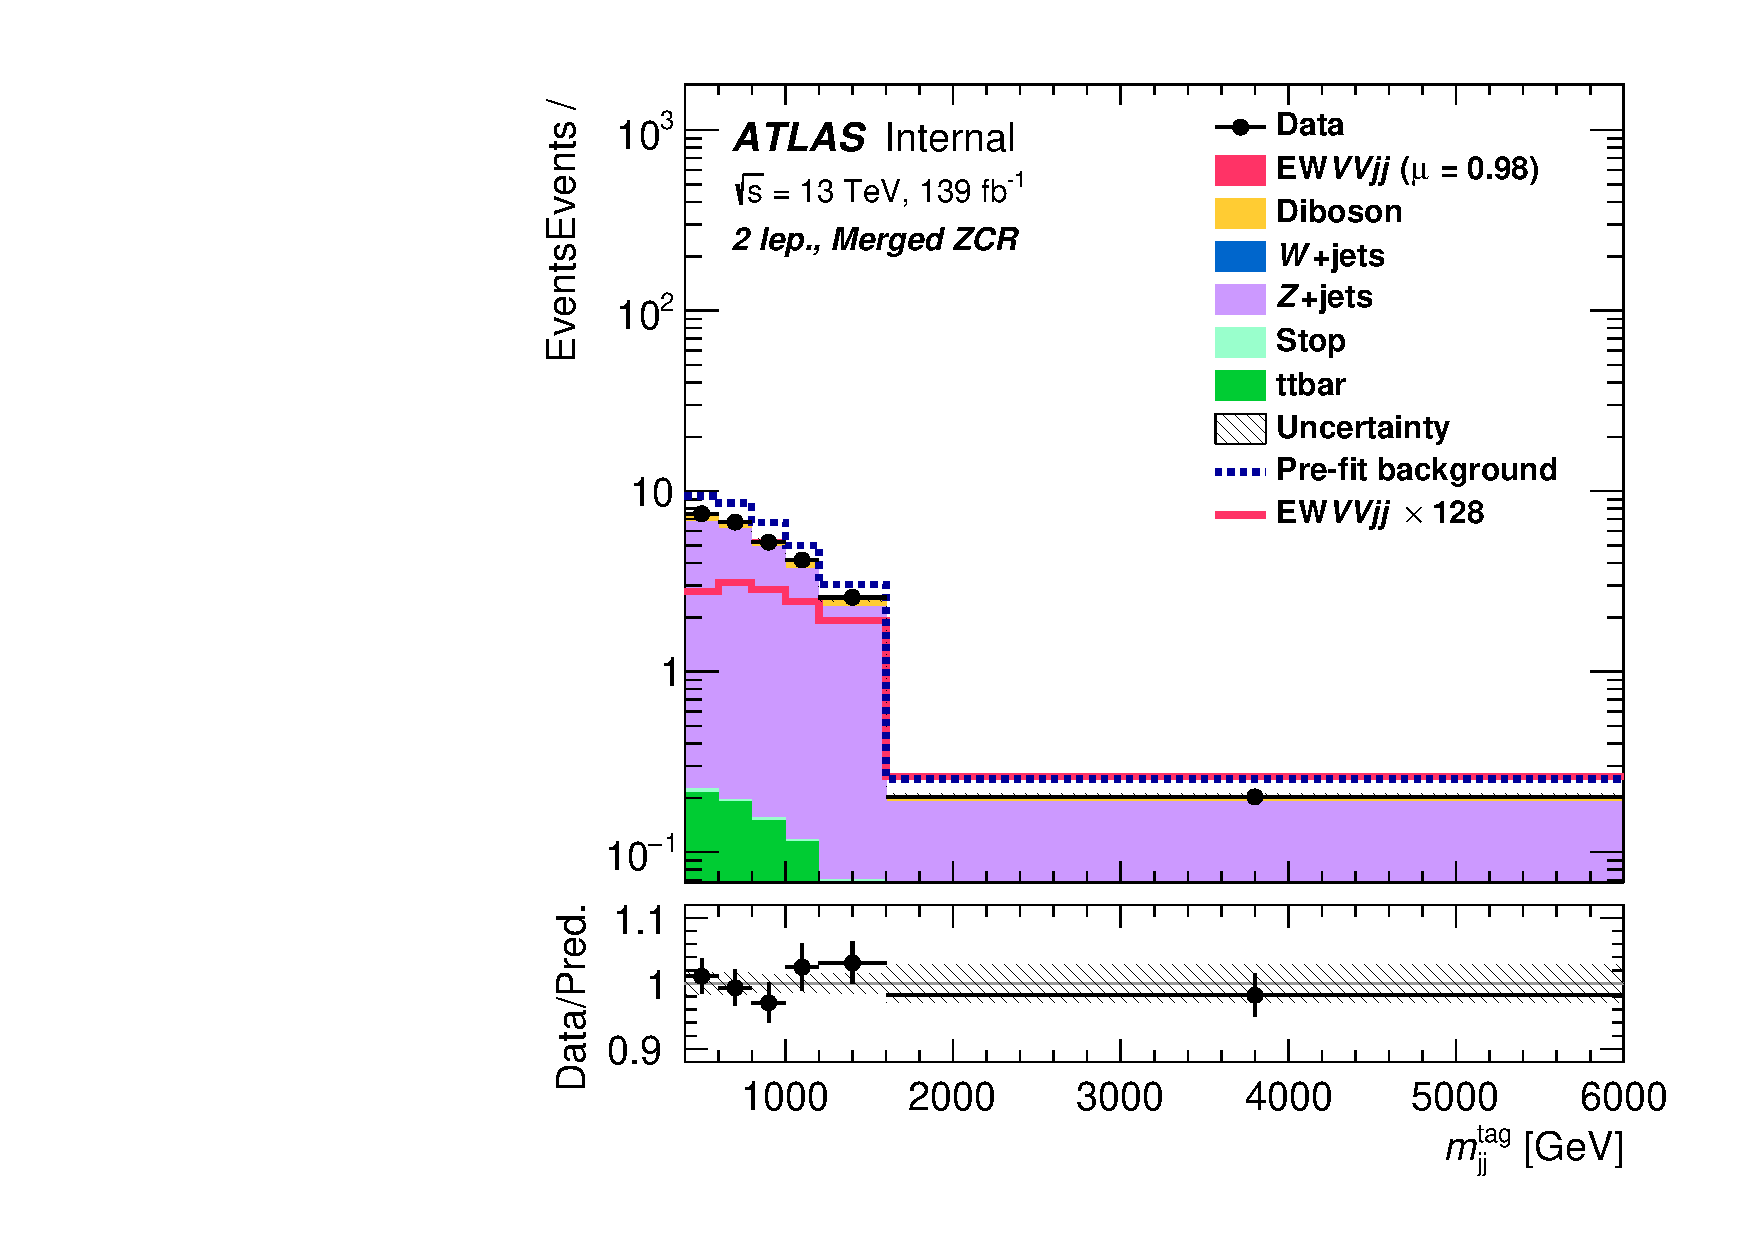
\includegraphics[width=0.45\textwidth]{figures/PostFit/Region_distMTagMerJets_DCRVjet_BMin0_J0_incJet1_L2_T0_incFat1_Y6051_incTag1_Fat1_GlobalFit_unconditionnal_mu1log}
      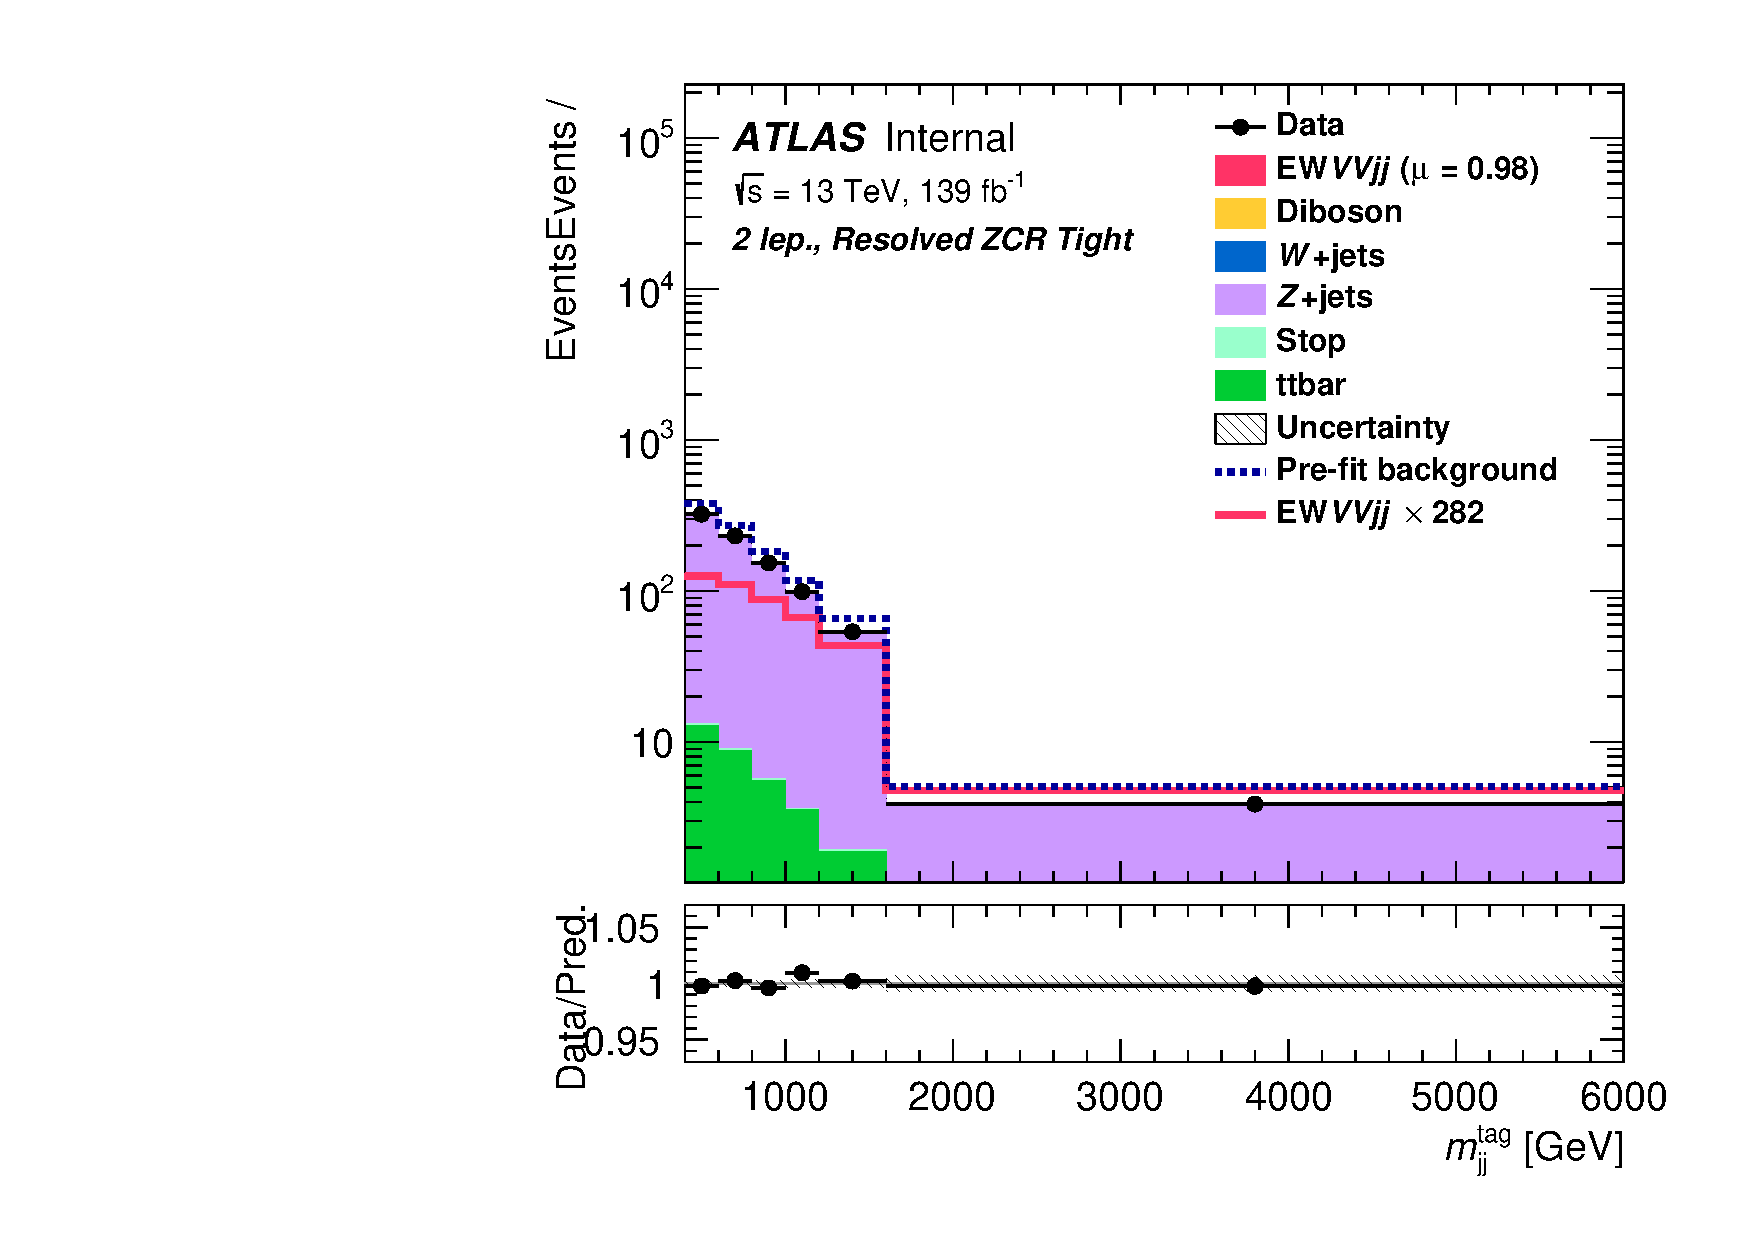
\includegraphics[width=0.45\textwidth]{figures/PostFit/Region_distMTagResJets_DCRVjetFid_BMin0_T0_Y6051_incTag1_J2_L2_incJet1_GlobalFit_unconditionnal_mu1log}
    \caption{Comparisons of the observed data and expected background distributions of $m^{tag}_{jj}$ in V+jets CRs in 0-lepton channel (1st line), 1-lepton channel (2nd line), and 2-lepton channel (3rd line). The EW VV+jj signal is filled on top of the fitted backgrounds, normalized to the signal yield extracted from the observed data ($\mu = 0.98$). The bottom panel show the ratio of the observed data to the post fit signal and background predictions.}
    \label{fig:postCR}
\end{figure}

\begin{figure}[H]
    \centering
    %1lep
    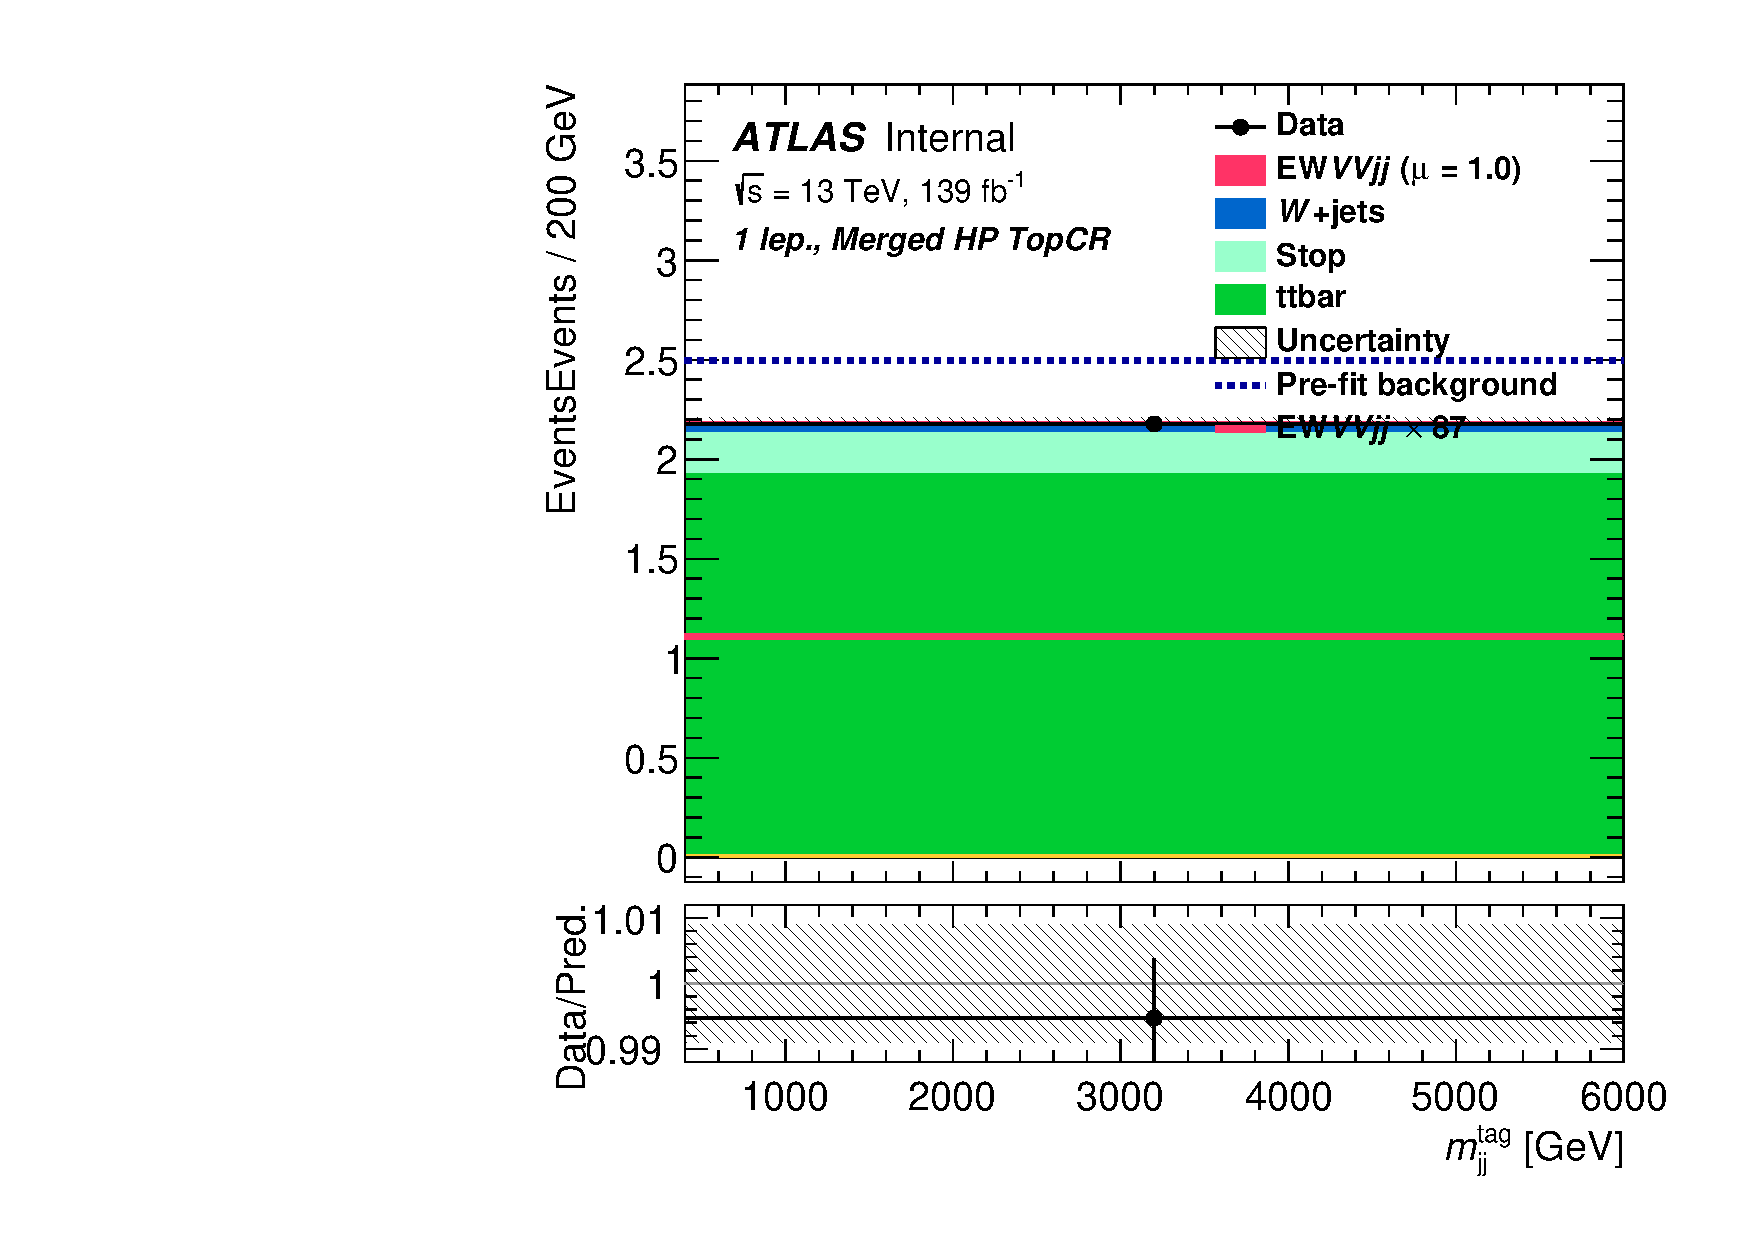
\includegraphics[width=0.45\textwidth]{figures/PostFit/Region_disttagMjj_DCRTopHP_BMin0_J0_incJet1_L1_T0_incFat1_Y6051_incTag1_Fat1_GlobalFit_unconditionnal_mu1}
    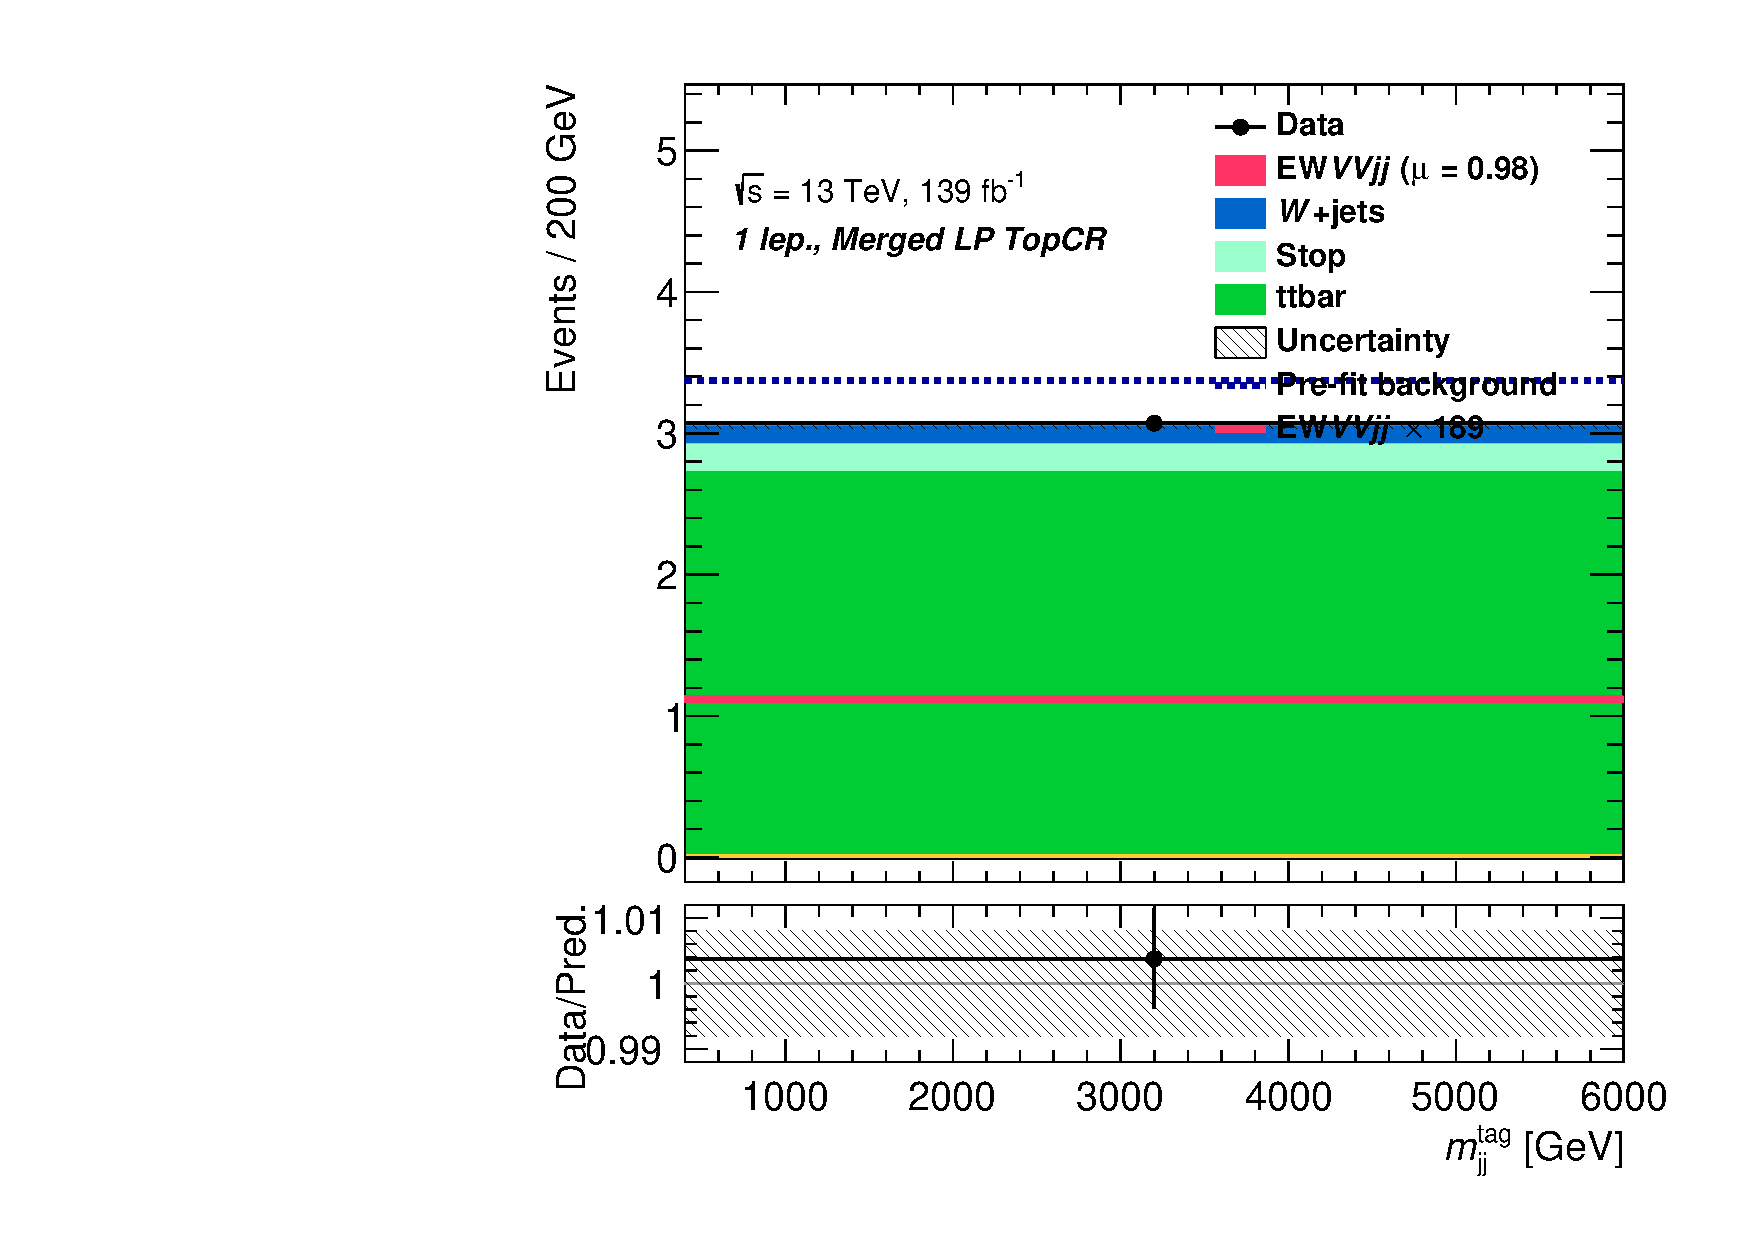
\includegraphics[width=0.45\textwidth]{figures/PostFit/Region_disttagMjj_DCRTopLP_BMin0_J0_incJet1_L1_T0_incFat1_Y6051_incTag1_Fat1_GlobalFit_unconditionnal_mu1}
    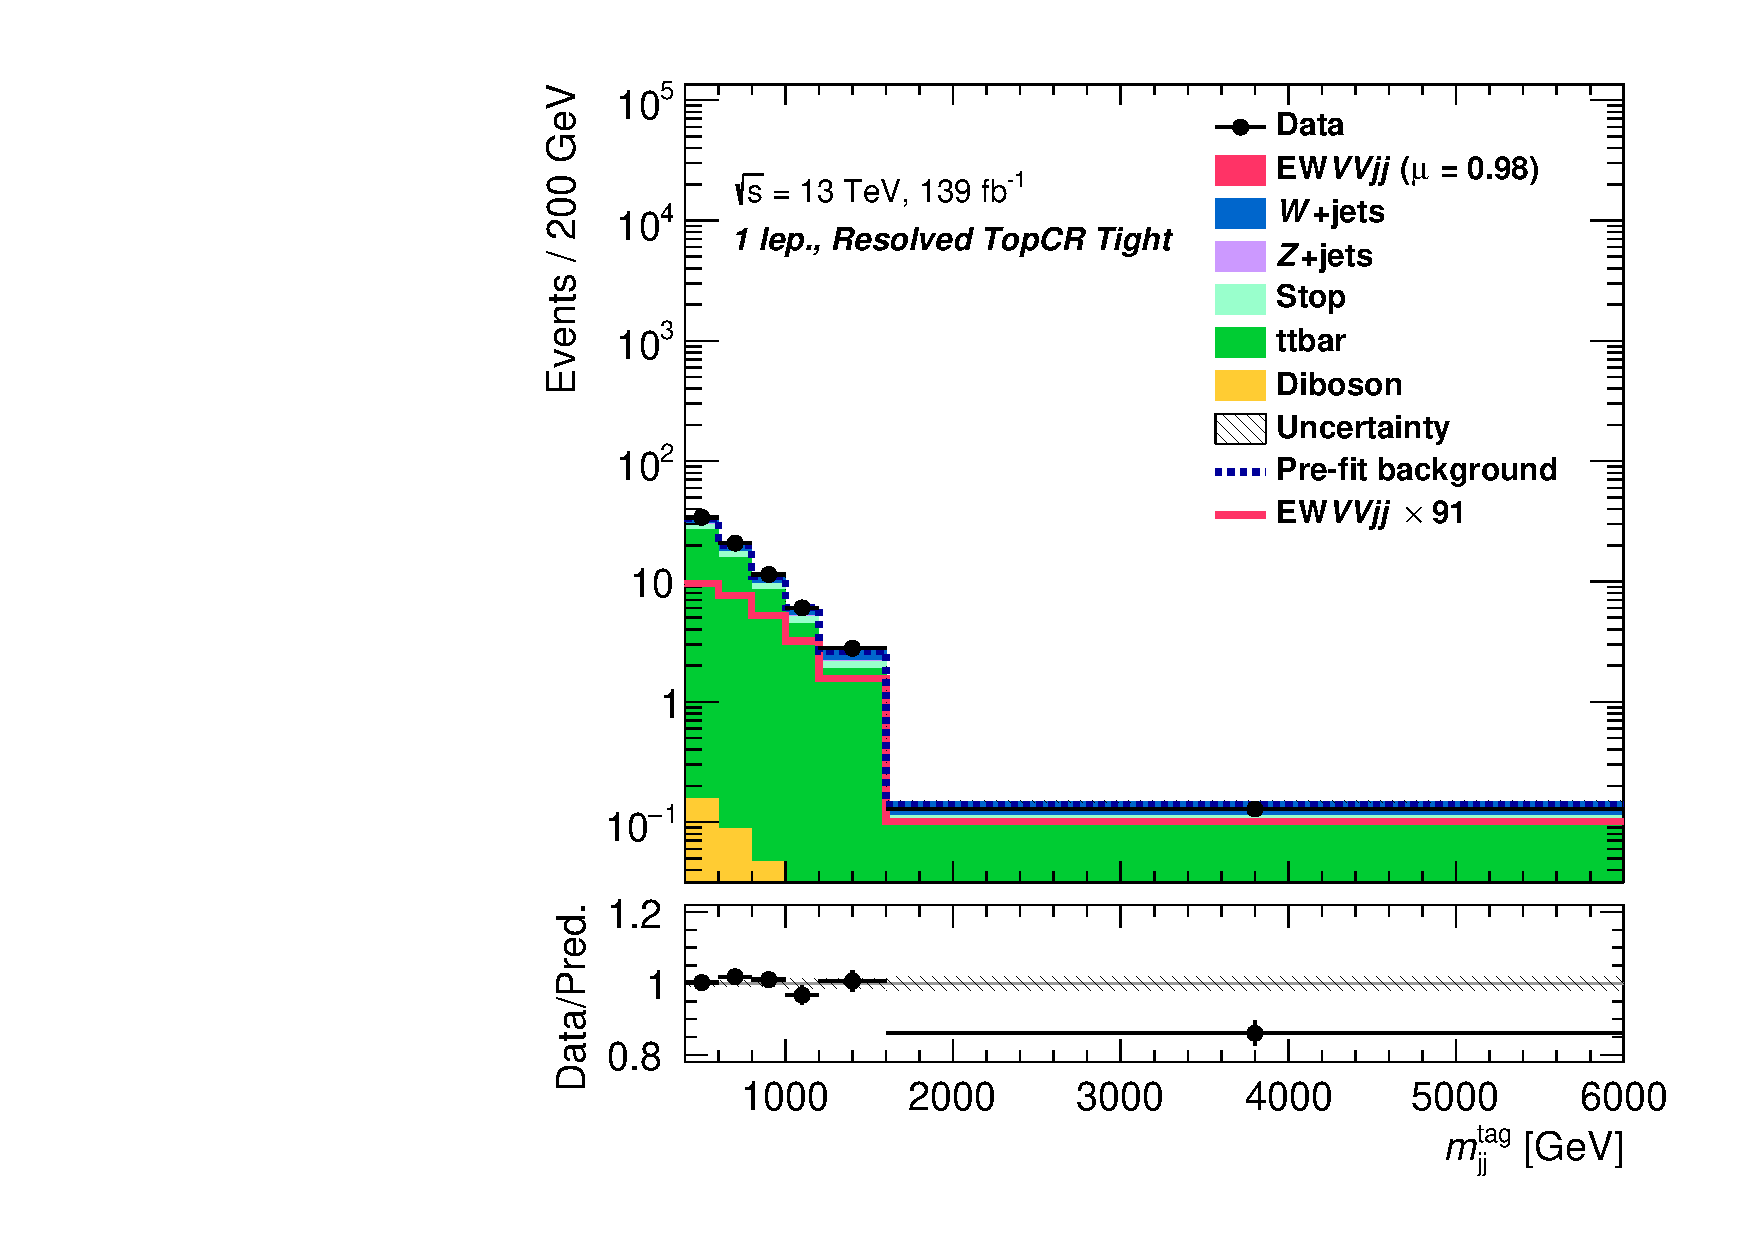
\includegraphics[width=0.45\textwidth]{figures/PostFit/Region_disttagMjj_DCRTopTight_BMin0_T0_Y6051_incTag1_J2_L1_incJet1_GlobalFit_unconditionnal_mu1log} 
    \caption{Comparisons of the observed data and expected background distributions of $m^{tag}_{jj}$ in Top CRs in 1-lepton channel.  The EW VV+jj signal is filled on top of the fitted backgrounds, normalized to the signal yield extracted from the observed data ($\mu = 0.98$). The bottom panel show the ratio of the observed data to the post fit signal and background predictions.}
    \label{fig:postCRTop}
\end{figure}

%\noindent\textbf{\sf{RNN score distributions at SRs after fitting}}\\
\subsection{RNN score distributions at SRs after fitting}
The RNN score distributions in each SRs after fitting are shown in figure~\ref{fig:postSR0lep}, \ref{fig:postSR1lep}, \ref{fig:postSR2lep}.
Basically the MCs match to the data well.

%signal region
\begin{figure}[H]
    \centering
    %0lep
    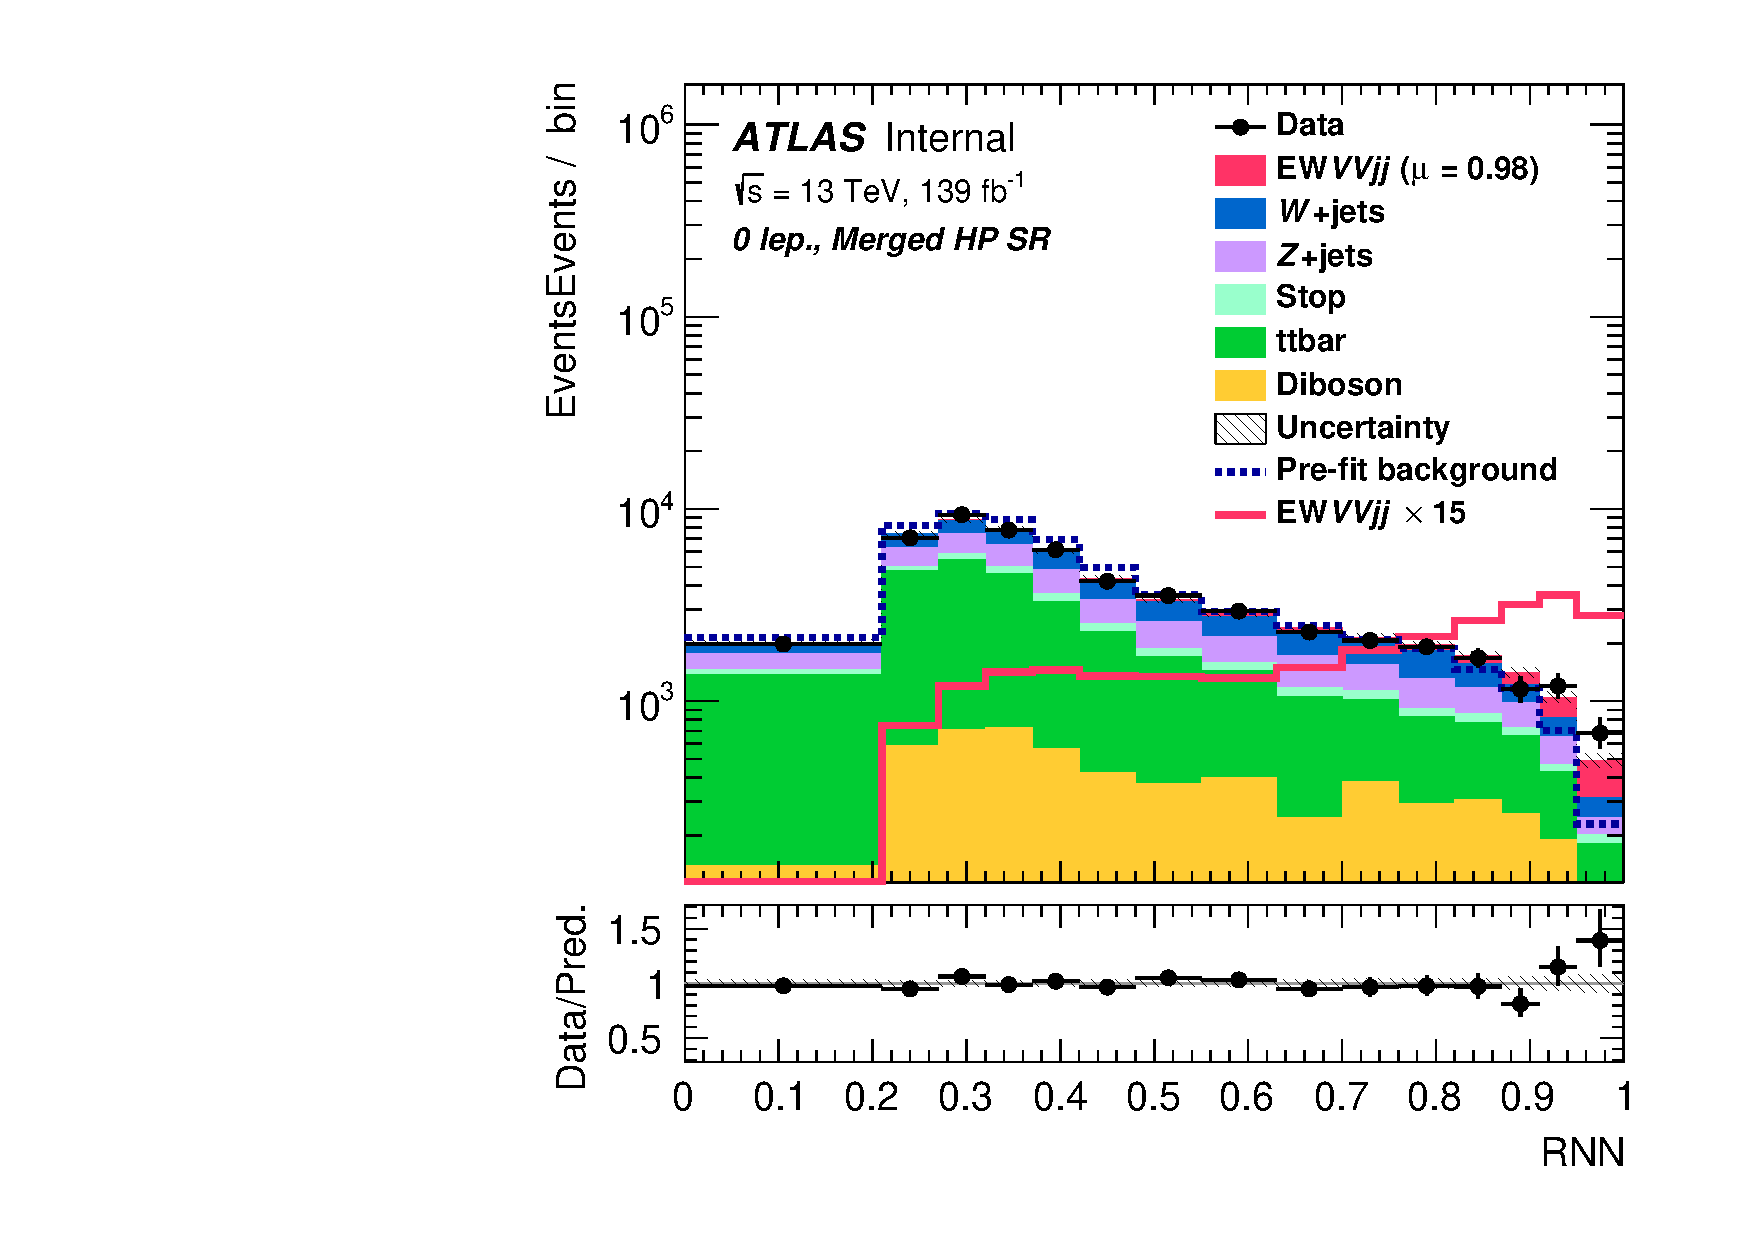
\includegraphics[width=0.45\textwidth]{figures/PostFit/Region_distRNN_DSRVBSHP_BMin0_J0_incJet1_L0_T0_incFat1_Y6051_incTag1_Fat1_GlobalFit_unconditionnal_mu1log}
    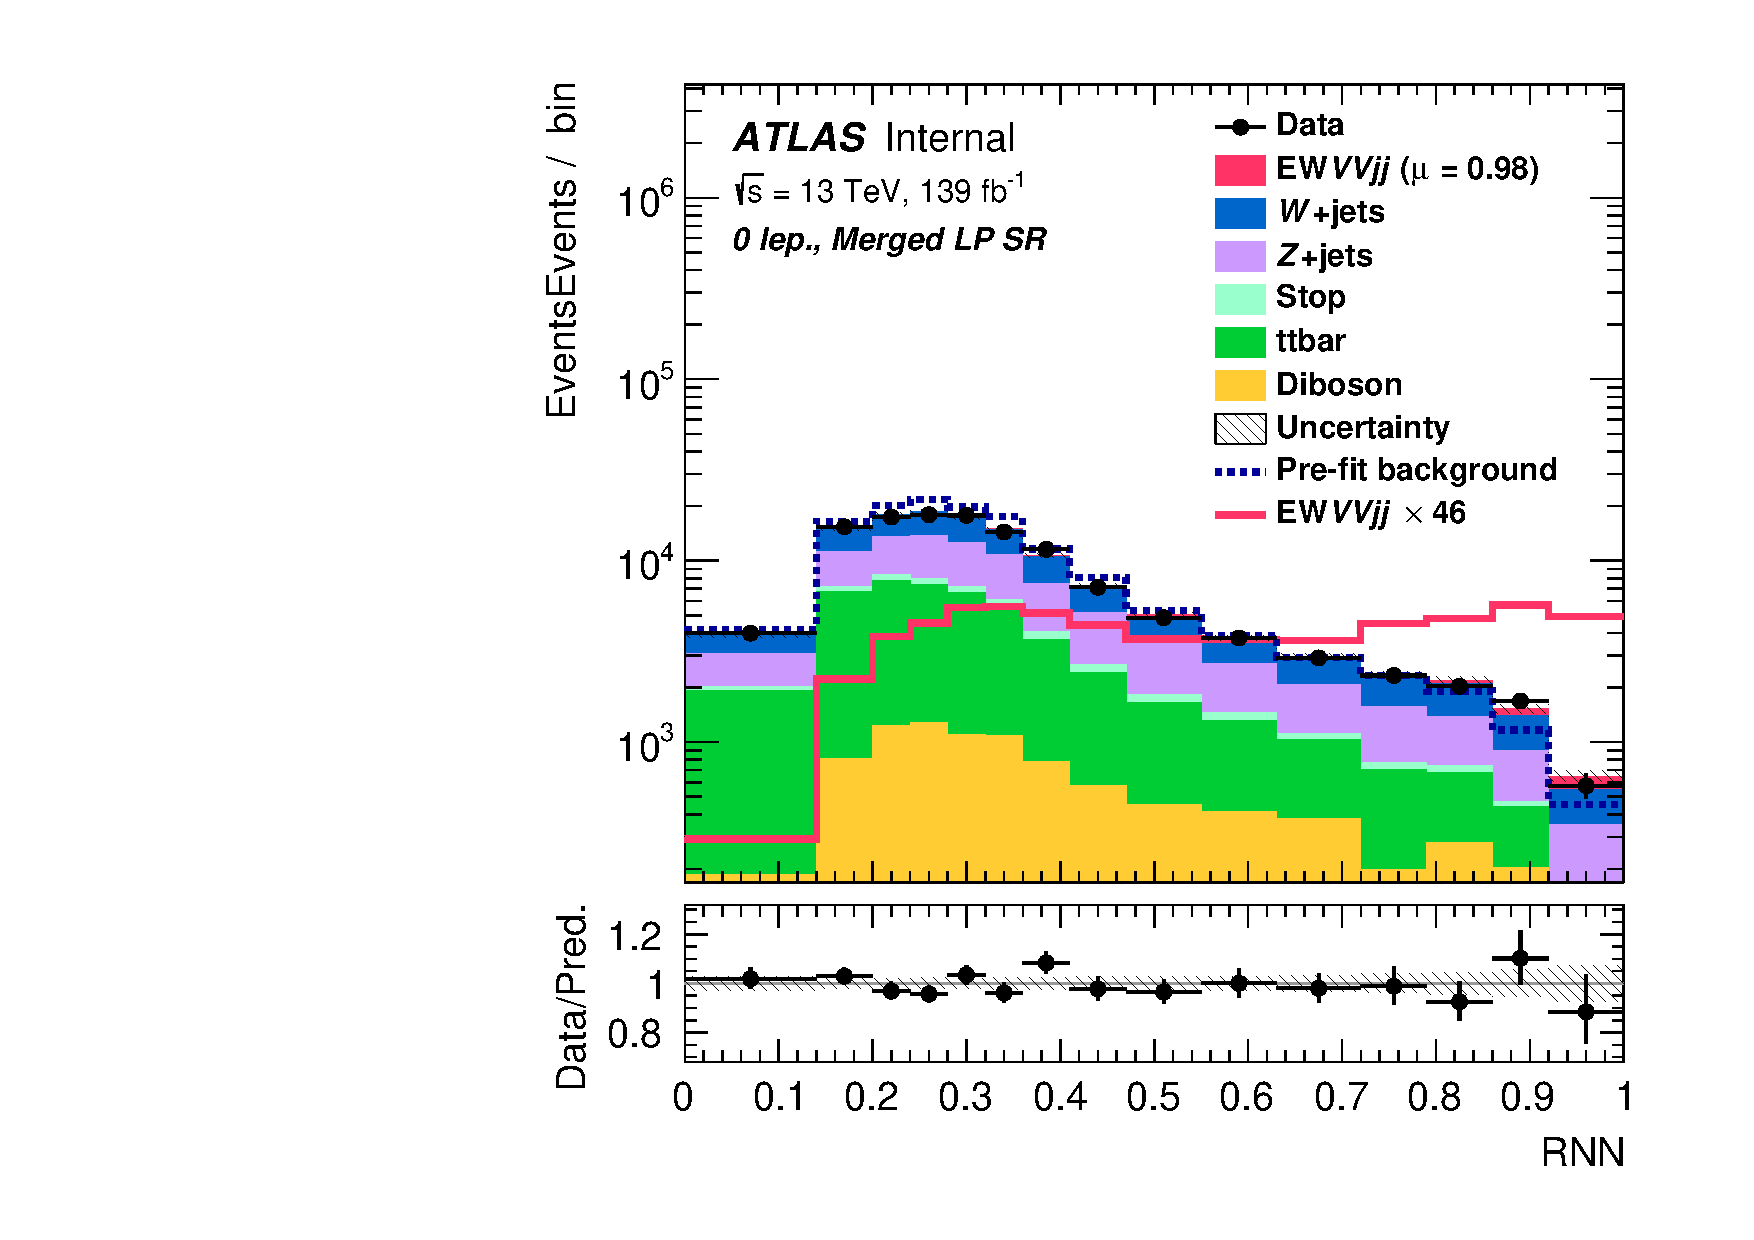
\includegraphics[width=0.45\textwidth]{figures/PostFit/Region_distRNN_DSRVBSLP_BMin0_J0_incJet1_L0_T0_incFat1_Y6051_incTag1_Fat1_GlobalFit_unconditionnal_mu1log}
    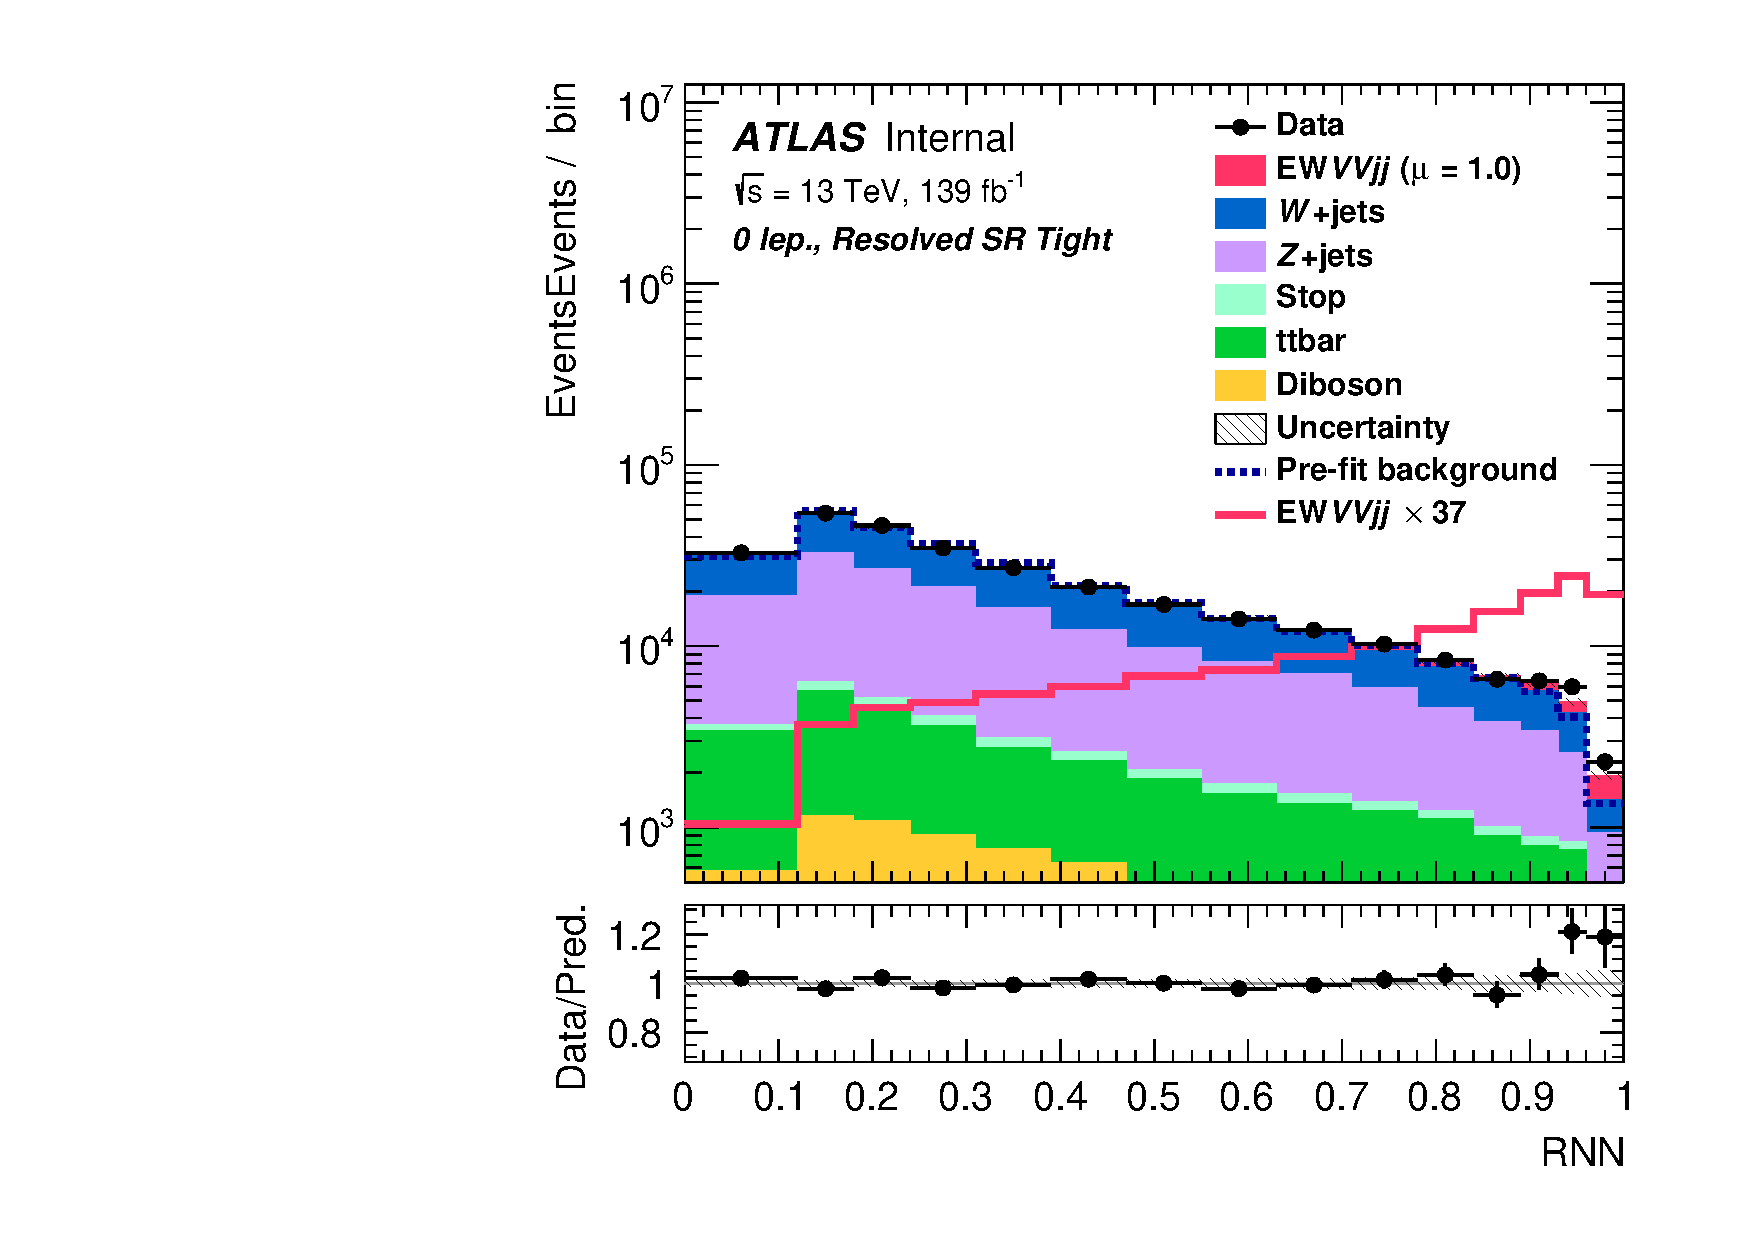
\includegraphics[width=0.45\textwidth]{figures/PostFit/Region_distRNN_DSRVBSFid_BMin0_T0_Y6051_incTag1_J2_L0_incJet1_GlobalFit_unconditionnal_mu1log}
      \caption{SR}
      \label{fig:postSR0lep}
\end{figure}
\begin{figure}[H]
    \centering
    %1lep
    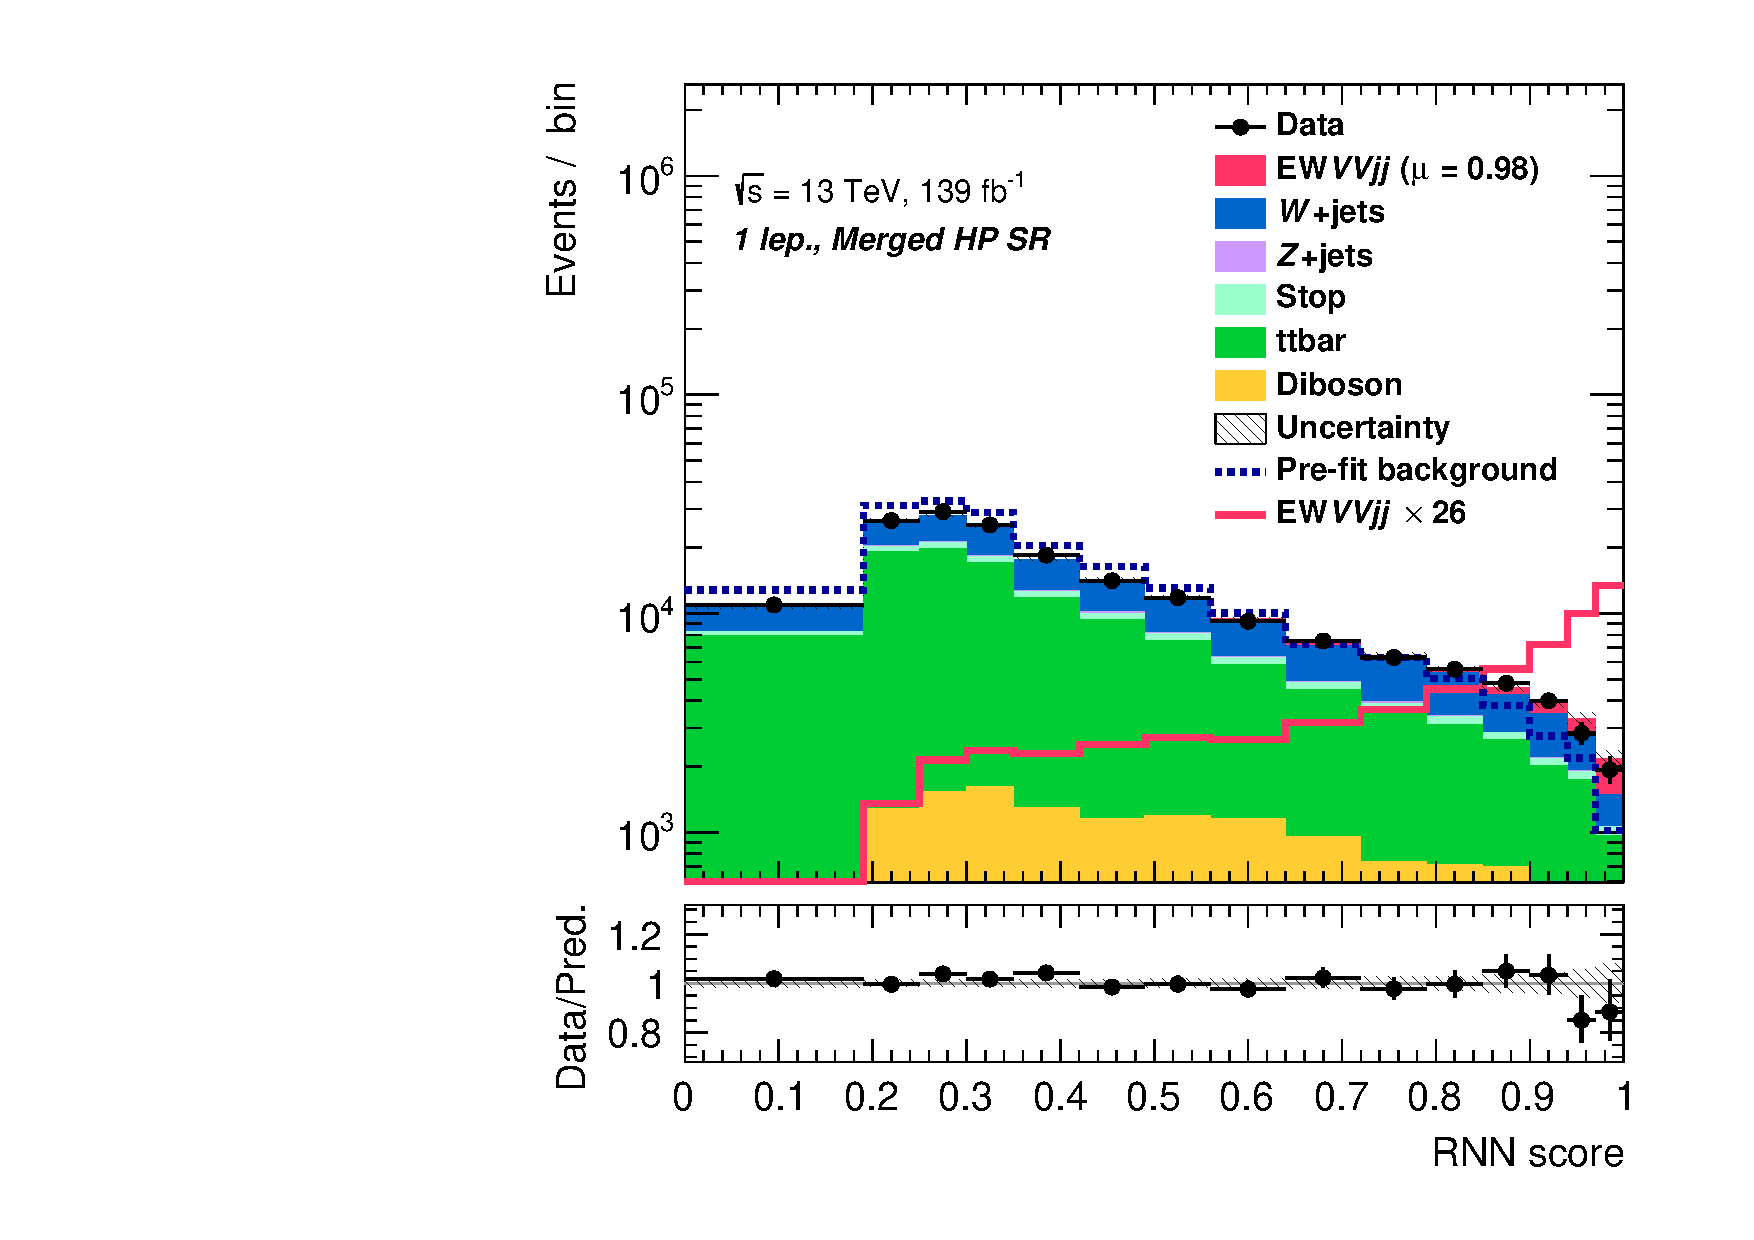
\includegraphics[width=0.45\textwidth]{figures/PostFit/Region_distRNN_DSRVBSHP_BMin0_J0_incJet1_L1_T0_incFat1_Y6051_incTag1_Fat1_GlobalFit_unconditionnal_mu1log}
    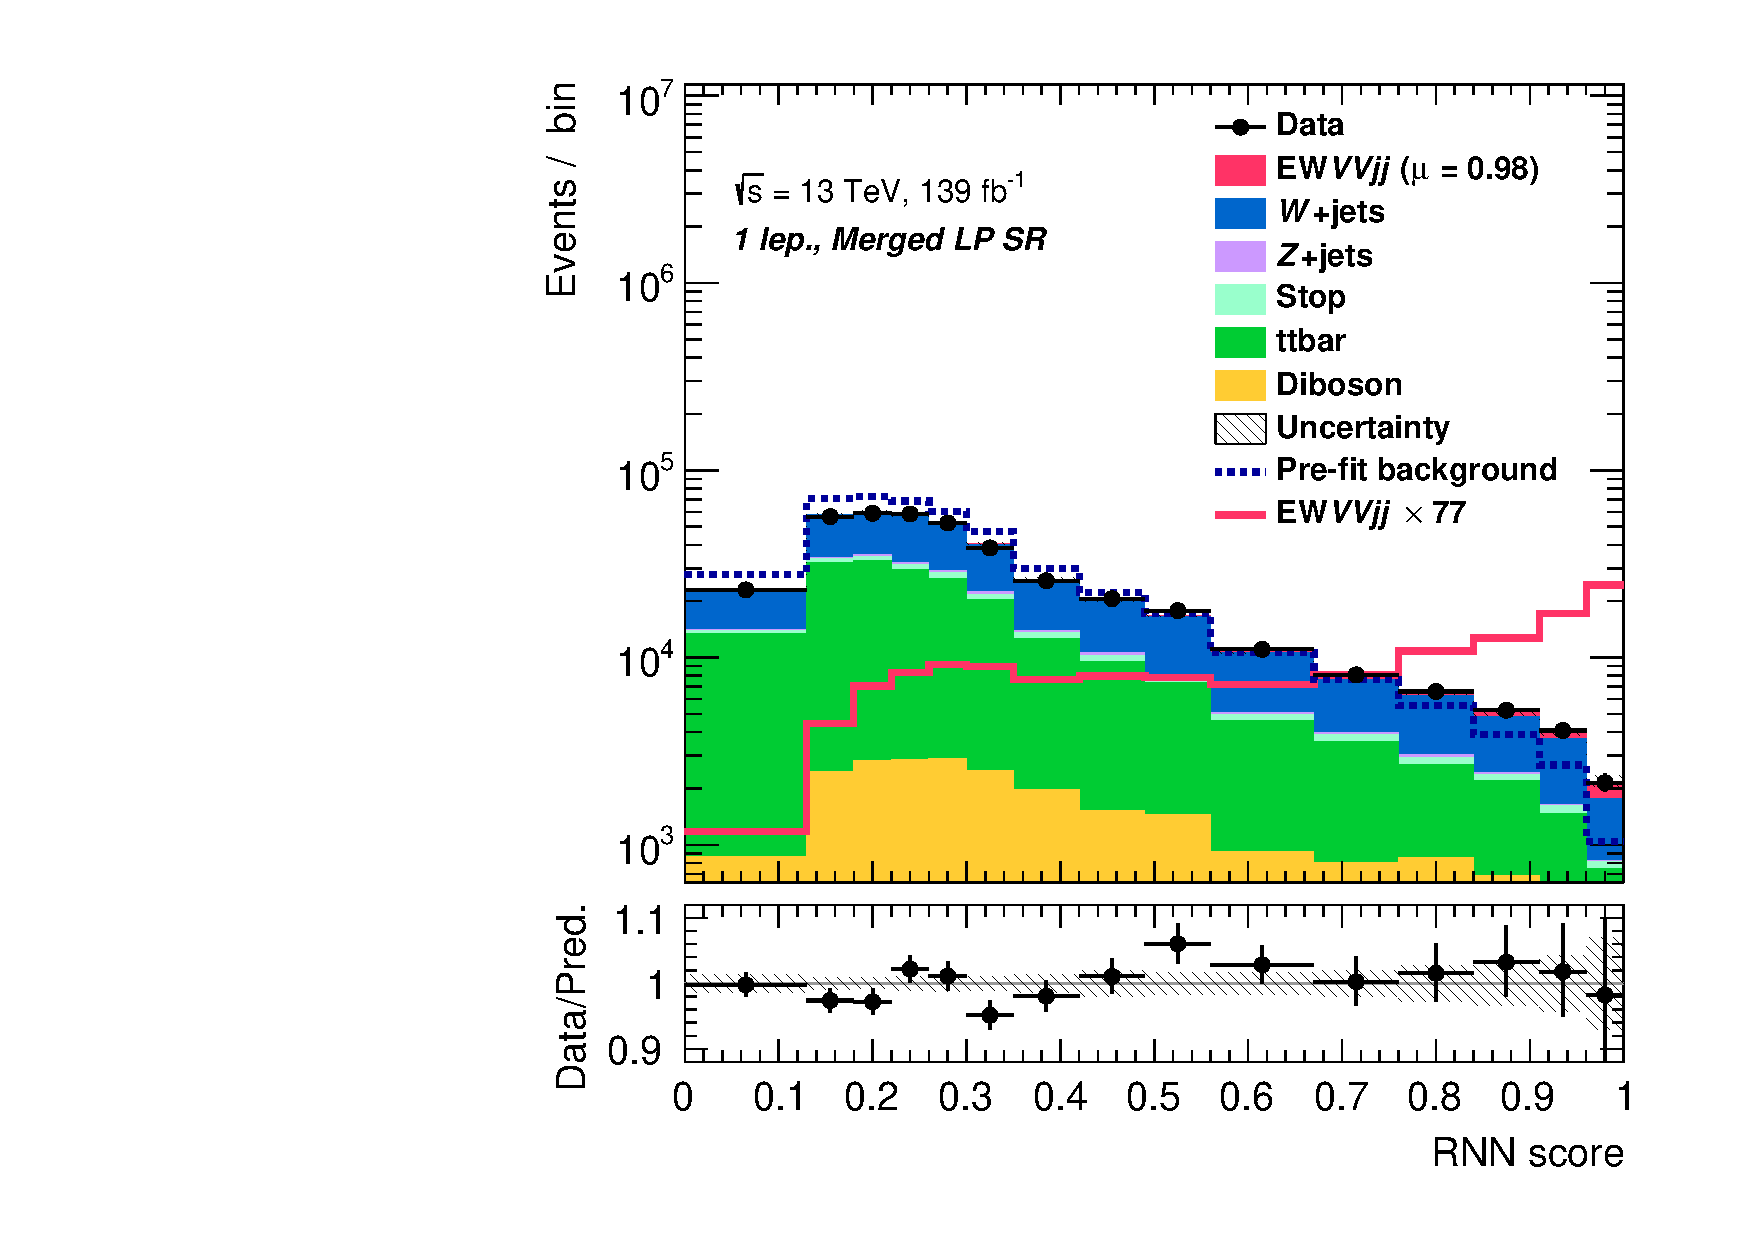
\includegraphics[width=0.45\textwidth]{figures/PostFit/Region_distRNN_DSRVBSLP_BMin0_J0_incJet1_L1_T0_incFat1_Y6051_incTag1_Fat1_GlobalFit_unconditionnal_mu1log}
    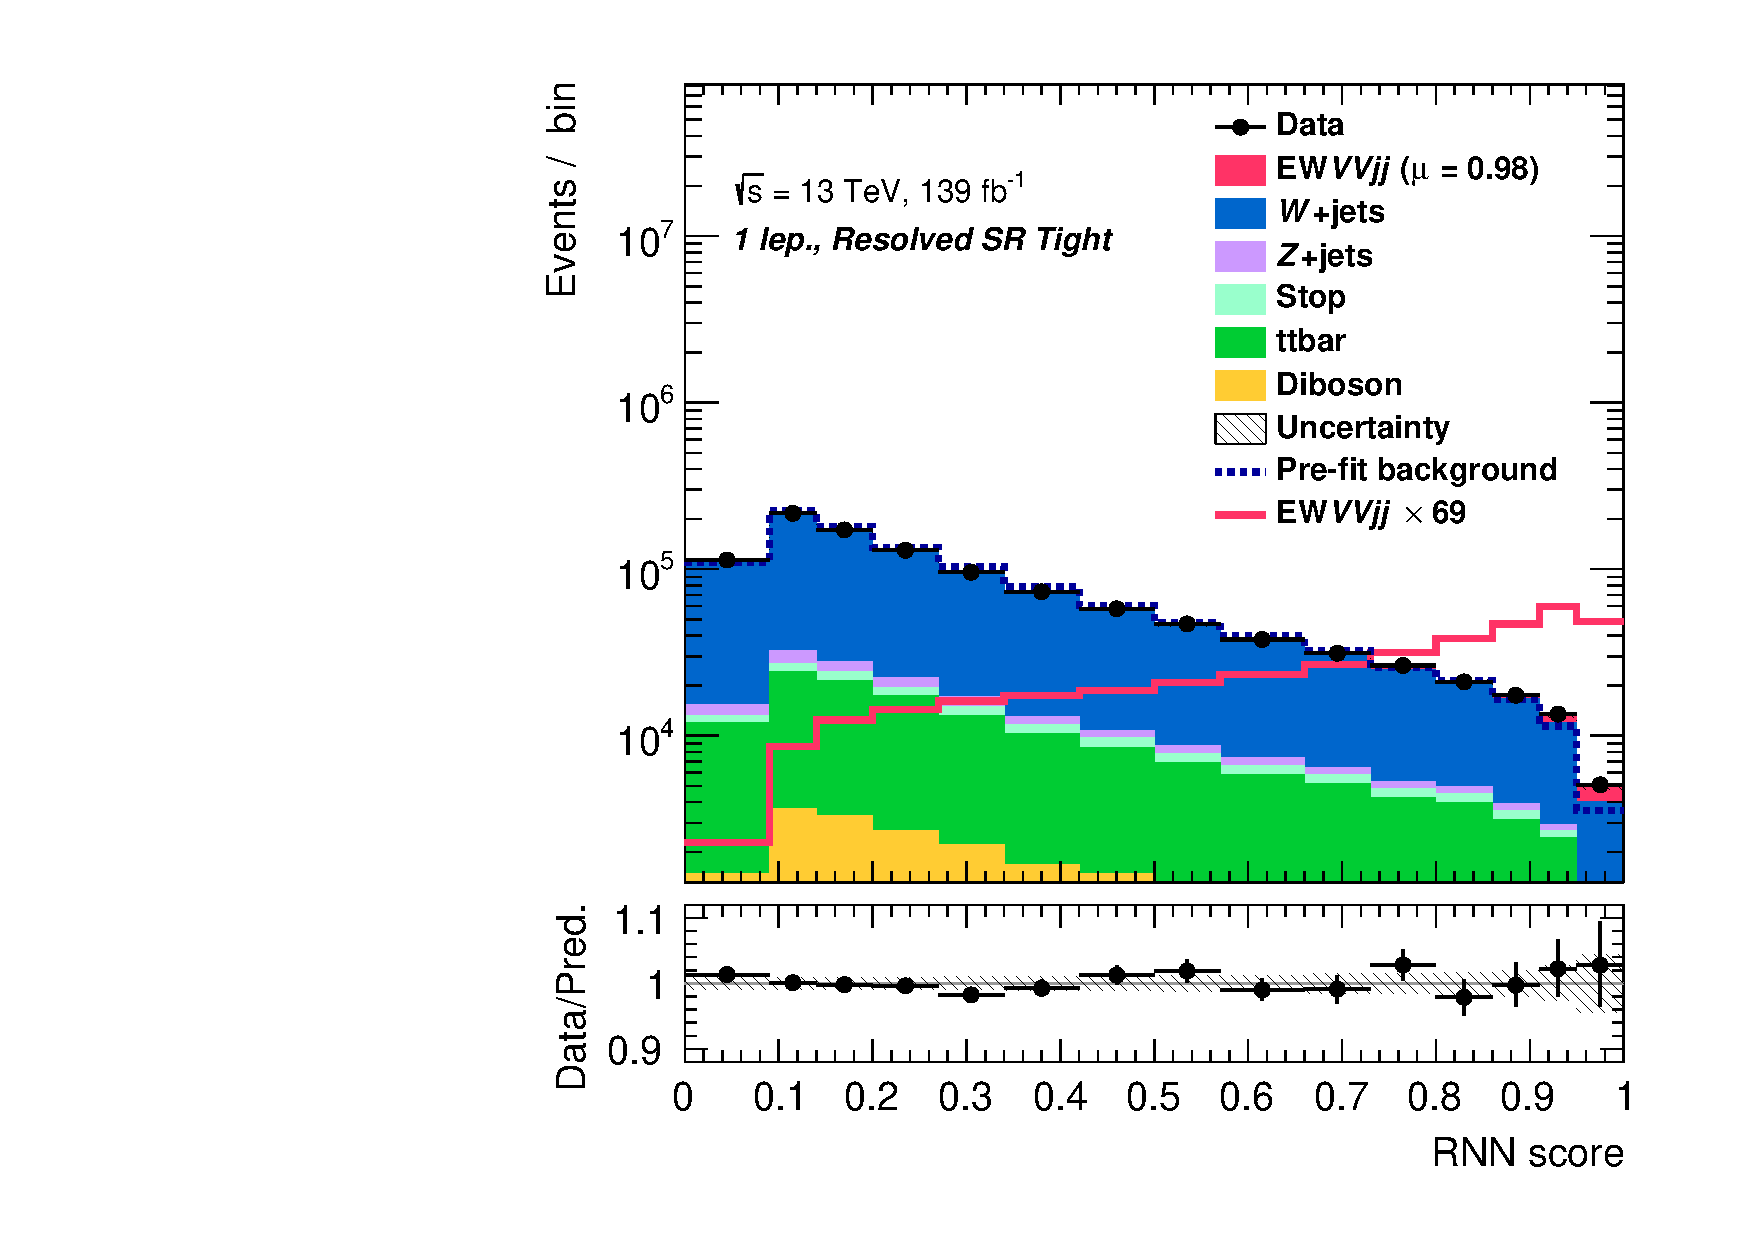
\includegraphics[width=0.45\textwidth]{figures/PostFit/Region_distRNN_DSRVBSTight_BMin0_T0_Y6051_incTag1_J2_L1_incJet1_GlobalFit_unconditionnal_mu1log}
      \caption{SR}
      \label{fig:postSR1lep}
\end{figure}
\begin{figure}[H]
    \centering
    %2lep
    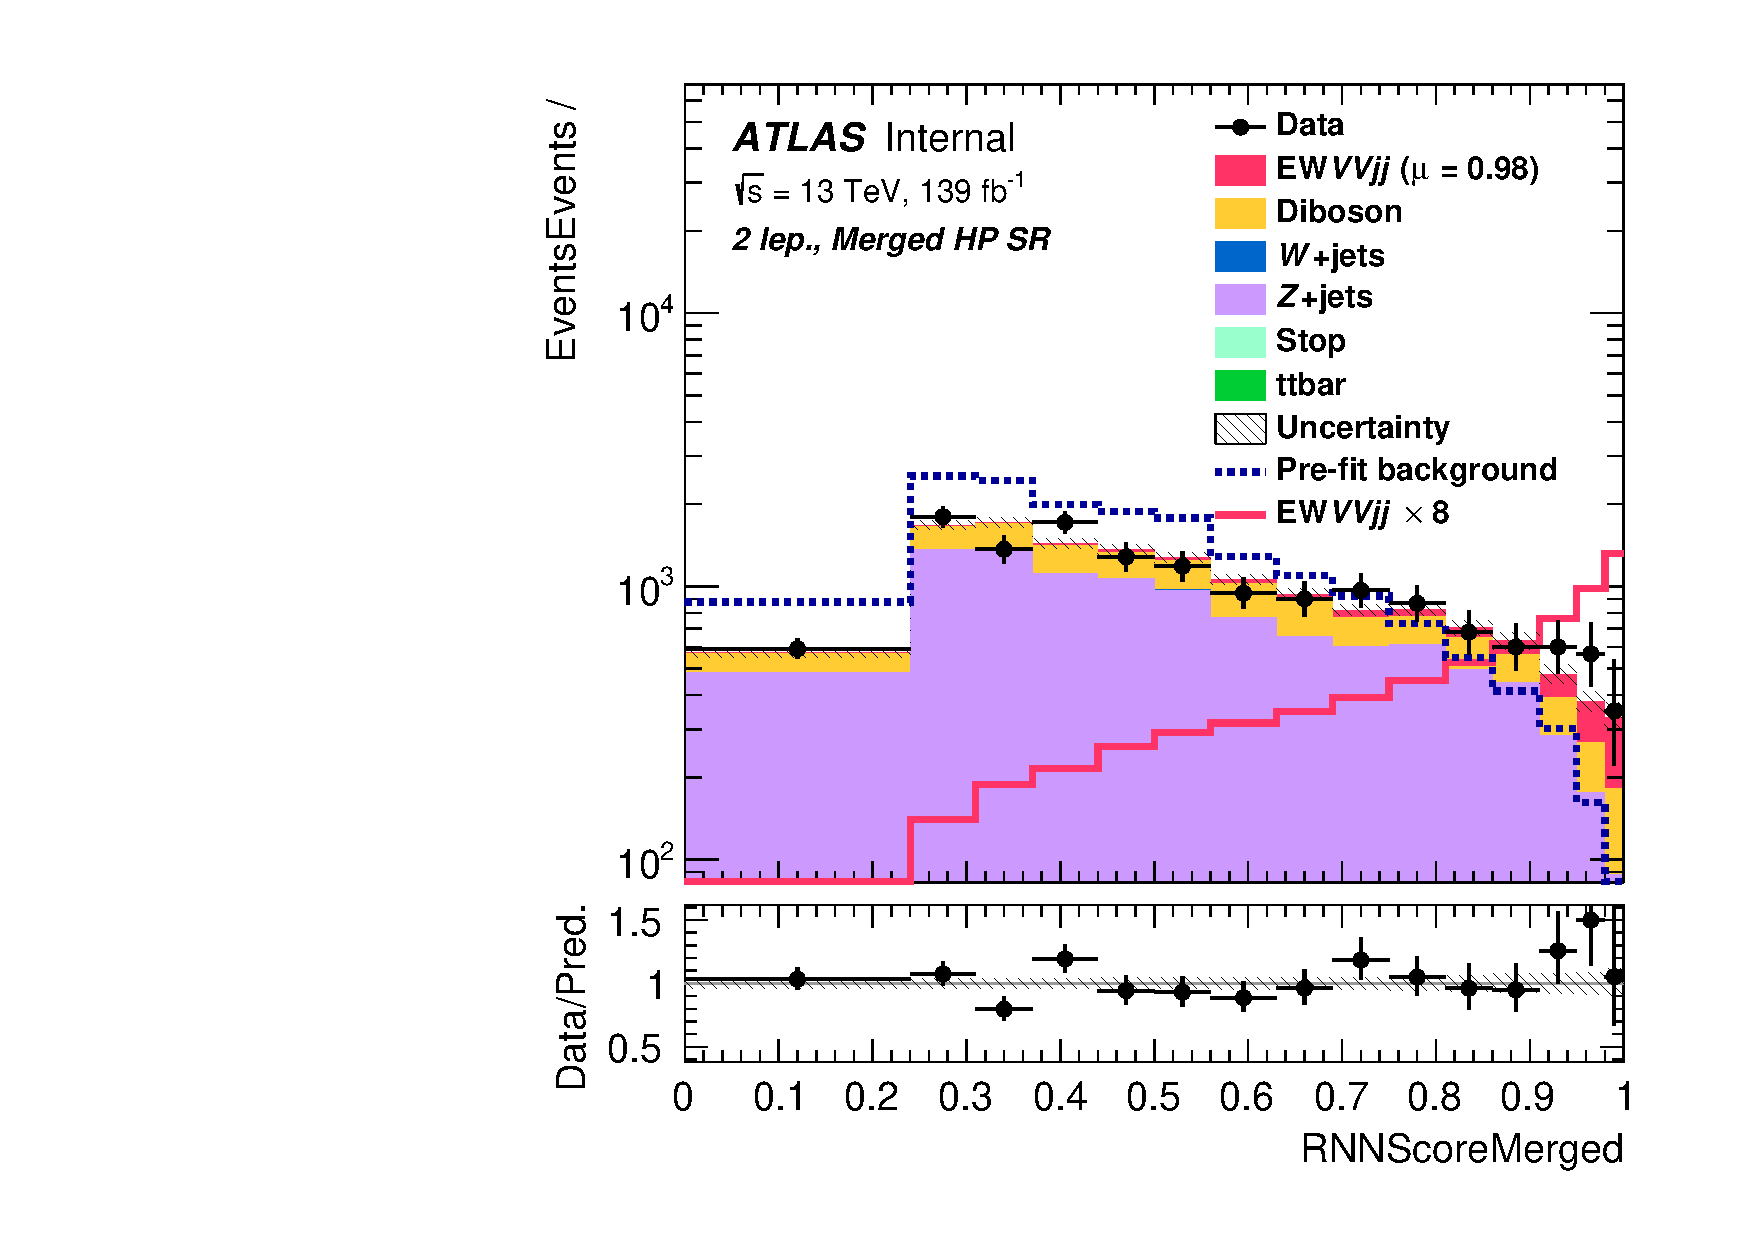
\includegraphics[width=0.45\textwidth]{figures/PostFit/Region_distRNNScoreMerged_DSRVBSHP_BMin0_J0_incJet1_L2_T0_incFat1_Y6051_incTag1_Fat1_GlobalFit_unconditionnal_mu1log}
    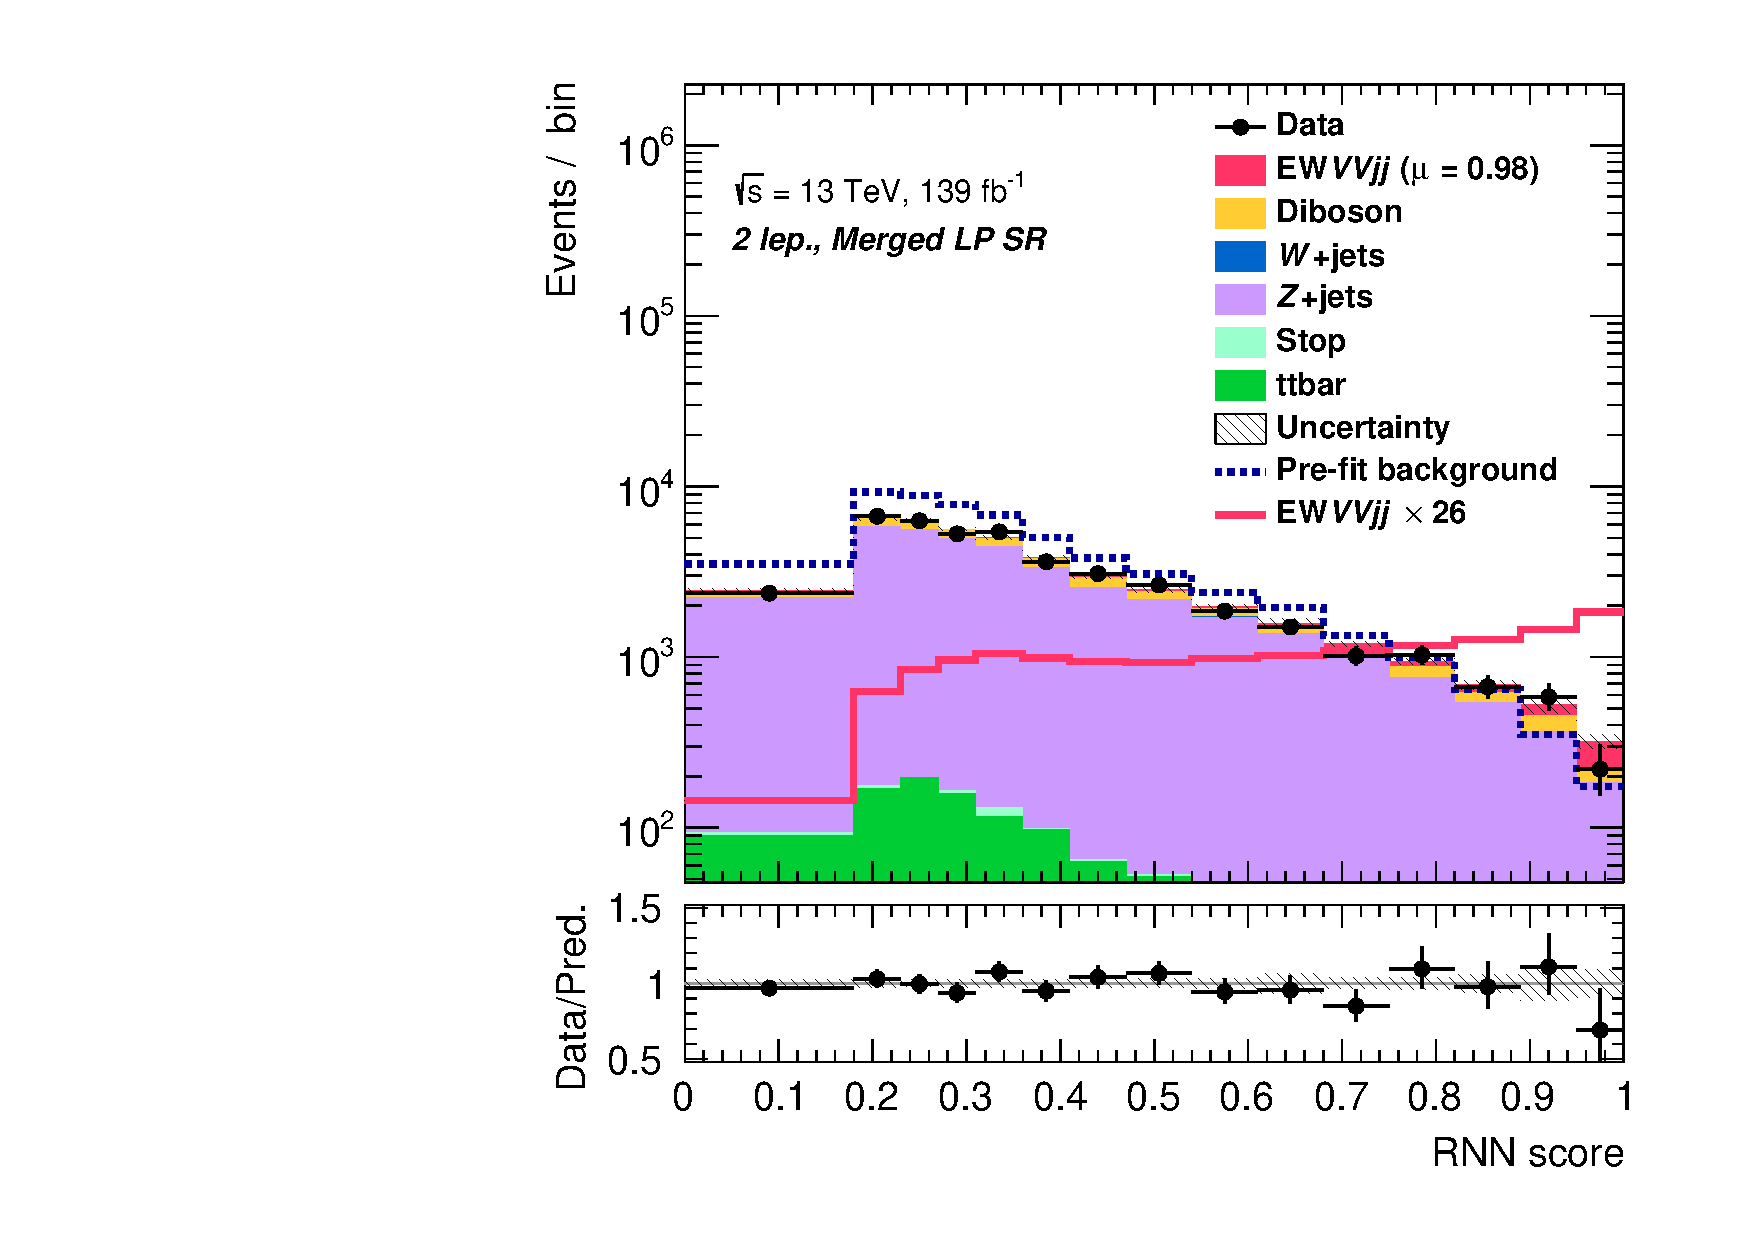
\includegraphics[width=0.45\textwidth]{figures/PostFit/Region_distRNNScoreMerged_DSRVBSLP_BMin0_J0_incJet1_L2_T0_incFat1_Y6051_incTag1_Fat1_GlobalFit_unconditionnal_mu1log}
    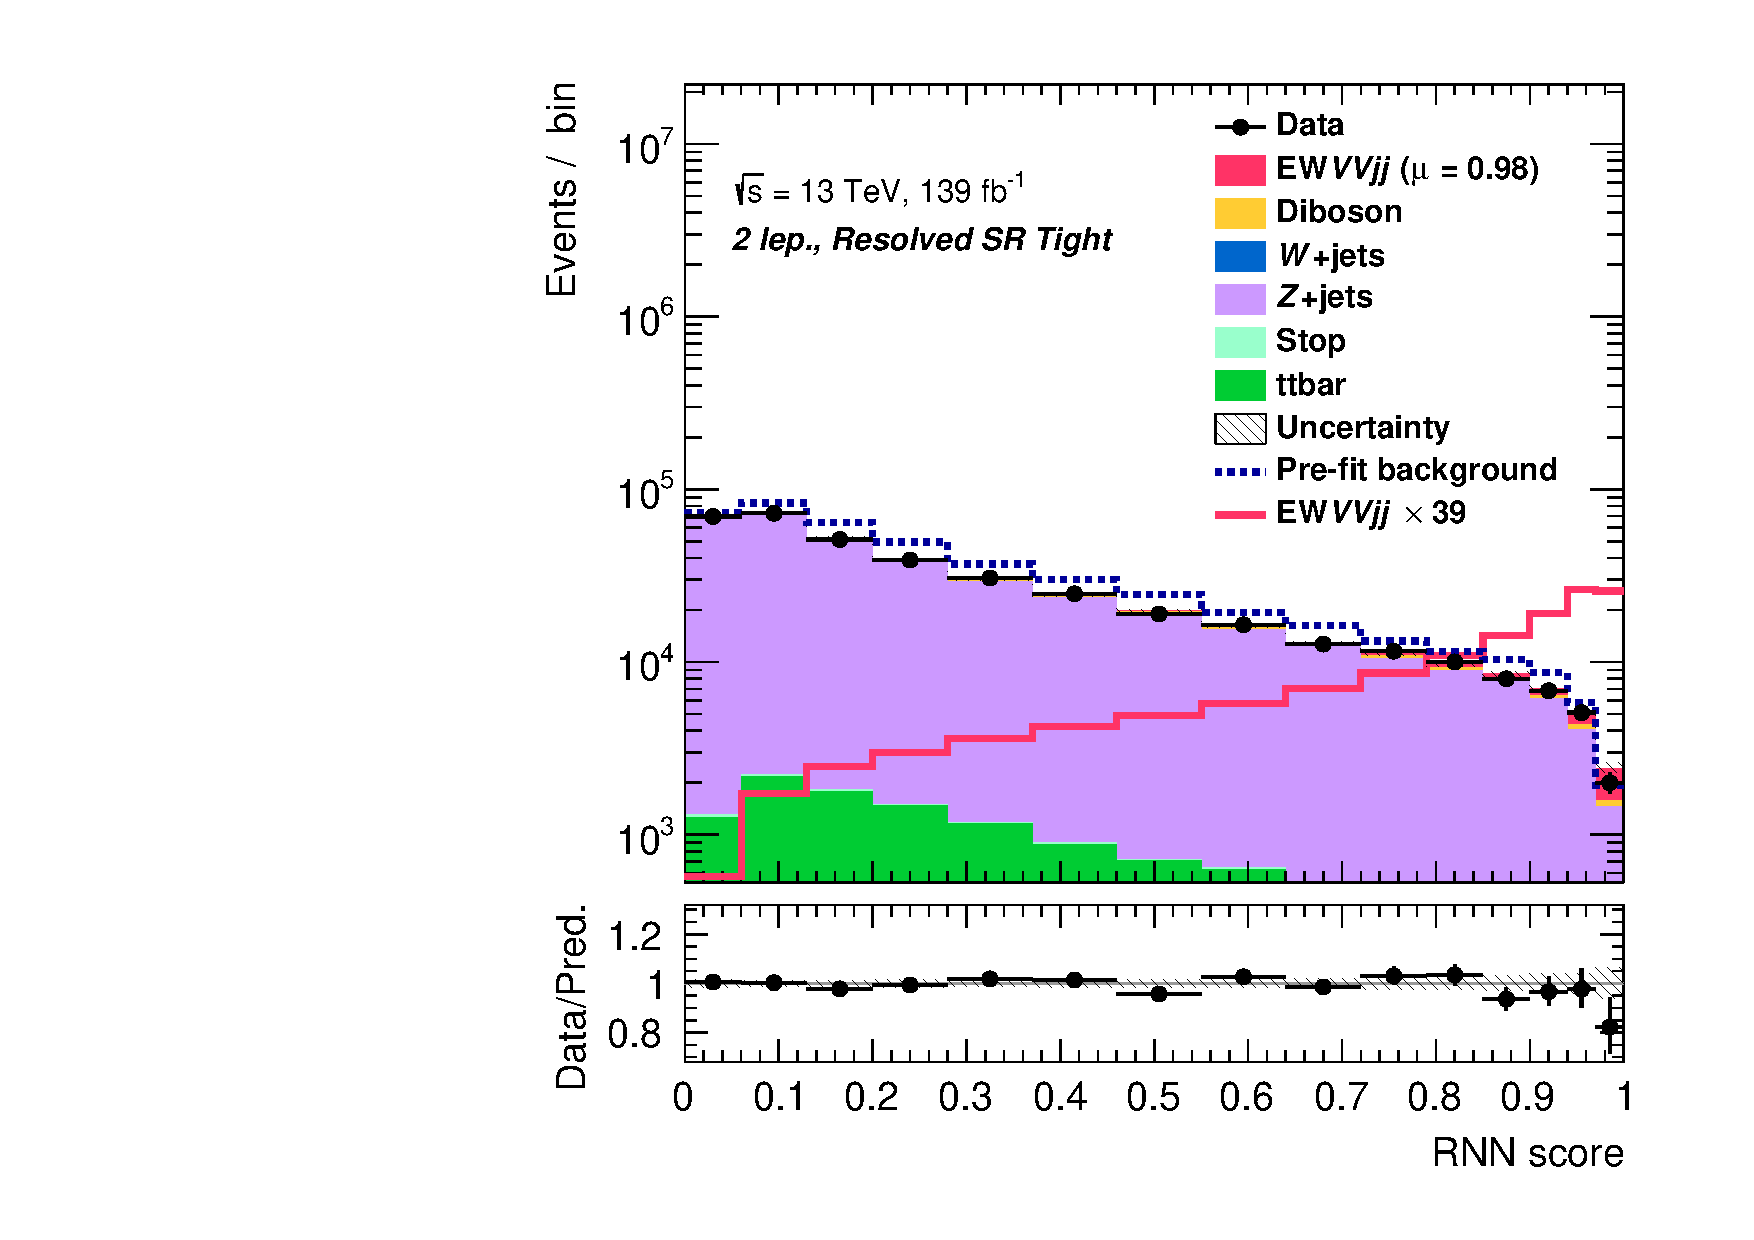
\includegraphics[width=0.45\textwidth]{figures/PostFit/Region_distRNNScoreResolved_DSRVBSFid_BMin0_T0_Y6051_incTag1_J2_L2_incJet1_GlobalFit_unconditionnal_mu1log}
    \caption{SR}
    \label{fig:postSR2lep}
\end{figure}

\section{Event yields after fitting}
\label{sec:eventyields}

The observed event yields after fitting is shown in table~\ref{}.
All the observed events yields in each region are compatible with the SM expectations.
%event yields
The summary of the normalization factor for each background component is shown in table~\ref{}. 
The summary of each normalization factor extracted from the fitting is shown in table~\ref{}.
%norm factors

\section{Impact of nuisance parameters on signal strength}

%\begin{itemize}
%       \item \texttt{SysTheoryQCD\_Z} 
%        This is the QCD scale uncertainty for the Z+jets background sample. This comes from the %large shape variation in the resolved SR. The input variations are shown in Figure and Figure %in the merged and resolved SRs. \\
%       \item \texttt{MJJREWEIGHT\_100per\_L2\_Fat1} 
%       \item \texttt{MJJREWEIGHT\_100per\_L2\_J2} \\
%       These are the $m^{tag}_{jj}$ reweighting uncertainties for merged and resolved regions. %We expect the large constraints for these uncertainties since these are taken as 100\% %uncertainties.Therefore CRs have large variations and constraints this systematics %uncertainties. \\
%       \item \texttt{SysMODEL\_Z\_MGPy8} \\
%       This is the shape difference between Sherpa Z+jets samples (after the \mjjtag reweighting %applied)and the MadGraph Z+jets samples (no \mjjtag reweighting applied). \\
%       These are expected since there is a well-known large modelling difference between two %generators. \\
%       \item \texttt{SysJET\_Pileup\_OffsetMu} \\
%       This is pile-up related uncertainty.
%       This systematic uncertainty is expected to have a large shape effect on the forward jets.
%%       \\
 %      \item \texttt{SysFATJET\_FatJetTagSF\_Gammajet\_Modelling} \\
 %      This is the uncertainty related to the boosted tagger SF efficiency.
 %      We can see this pull since this uncertainty has a large effect in Merged CR. 
%\end{itemize}

%Some strong pulls (1~$\sigma$ to 1.25~$\sigma$) are observed in the data fit in:
%\begin{itemize}
%    \item \texttt{TheoryQCD\_Z}\\
%    This pull mainly comes from the resolved SRs. Since the impact of this pull is relaxed when %%the left-side bin is merged, this pull seems to comes from the descripance between data to MC i%%%n the RNN left-side bins.
   % \item \texttt{MODEL\_Z\_MGPy8}\\
   % This is coming from the difference in the generators. Since the modeling is better in the %alternative generator, MadGraph, this parameter is pulled a lot to fit to the data.
%\end{itemize}
%The other constraints or pulled (up to 1~$\sigma$) parameters are listed below:
%\begin{itemize}
%    \item \texttt{SysJET\_Pileup\_OffsetMu}\\
%    This is pileup-related uncertainty. This is expected to have a large shape effect on the %forward jet as well as for jet track multiplicity.
%    \item \texttt{SysFATJET\_FatJetTagSF\_Gammajet\_Modeling} \\
%    This is the uncertainty related to the boosted tagger SF efficiency. This pull can be seen %since this  uncertainty has a large effect in Merged CR.
%\end{itemize}

%\subsection{Nuisance Paremeter Correlations}
%The correlation matrix for the Asimov full-range fit for the parameters which has more than 1\% %correlations with any other operators are shown, without statistical uncertainties in each bin %is shown in Figure~\ref{fit_2lep_corr_all}. The strongest correlation of $\minus 78\%$ shows up %%%%between \texttt{MODEL\_Z\_MGPy8} and \texttt{MJJREWEIGHT\_100per\_L2\_J2}. These two par%ameters are both related to the mis-modelling of the Z+jets samples therefore should have cor%relations.
%The parameters which have significant (more than $\pm 30\%$) correlations with the POI %\texttt{$\mu\_$SemileptonicVBS} are:
%\begin{itemize}
%    \item \texttt{TheoryQCD\_Z} 
%    \item \texttt{MODEL\_Z\_MGPy8} \\
%\end{itemize}

%\begin{figure}[ht]
%      \centering
%        \includegraphics[width=\linewidth]%{figures/2lep/FitResults/corr_HighCorrNoMCStat_AsimovAllbins.pdf}%
      %  \caption{Correlations for unconditional fit ($\mu=1$) to asimov data in the full range, for the 2 lepton channel only.}
      % \label{fig:fit_2lep_corr_all}
%\end{figure}

%\section{Rankings}
Ranking plots for all nuisance parameters without the bin-wise statistical uncertainties are shown in Figure~\ref{fig:fit_2lep_ranking_all}. The ranking plot shows the nuisance parameters which have large impact on the sensitivity. The ranking is derived by doing the scans of the likelihood function. First the nominal fit is performed to find the global maximum in the likelihood, and the corresponding $\hat{\mu}$. Then one nuisance parameter is fixed and scanned while all other parameters are fitted again. The scan as a function of one parameter stops once the logarithm of the likelihood decreases by 1/2 compared to the global maximum. This point corresponds to the 1~$\sigma$ uncertainty. The change of the signal strength, which is plotted as $\Delta\mu$ is evaluated here.
This scan is done with both direction of the NP and repeated for all NPs.
The top-two parameters are NPs relates to the Z+jet modeling issue and seen to be pulled in the pull plots. Varying these parameter by $1\sigma$ changes the signal strength by $\Delta \hat{\mu} \simeq 0.2$. The parameters which have strong impacts and highly-ranked are consistent with the parameters having strong correlations with the POI in the correlation plot, Figure~\ref{fig:fit_2lep_corr_all}.
\begin{figure}[ht]
      \centering
        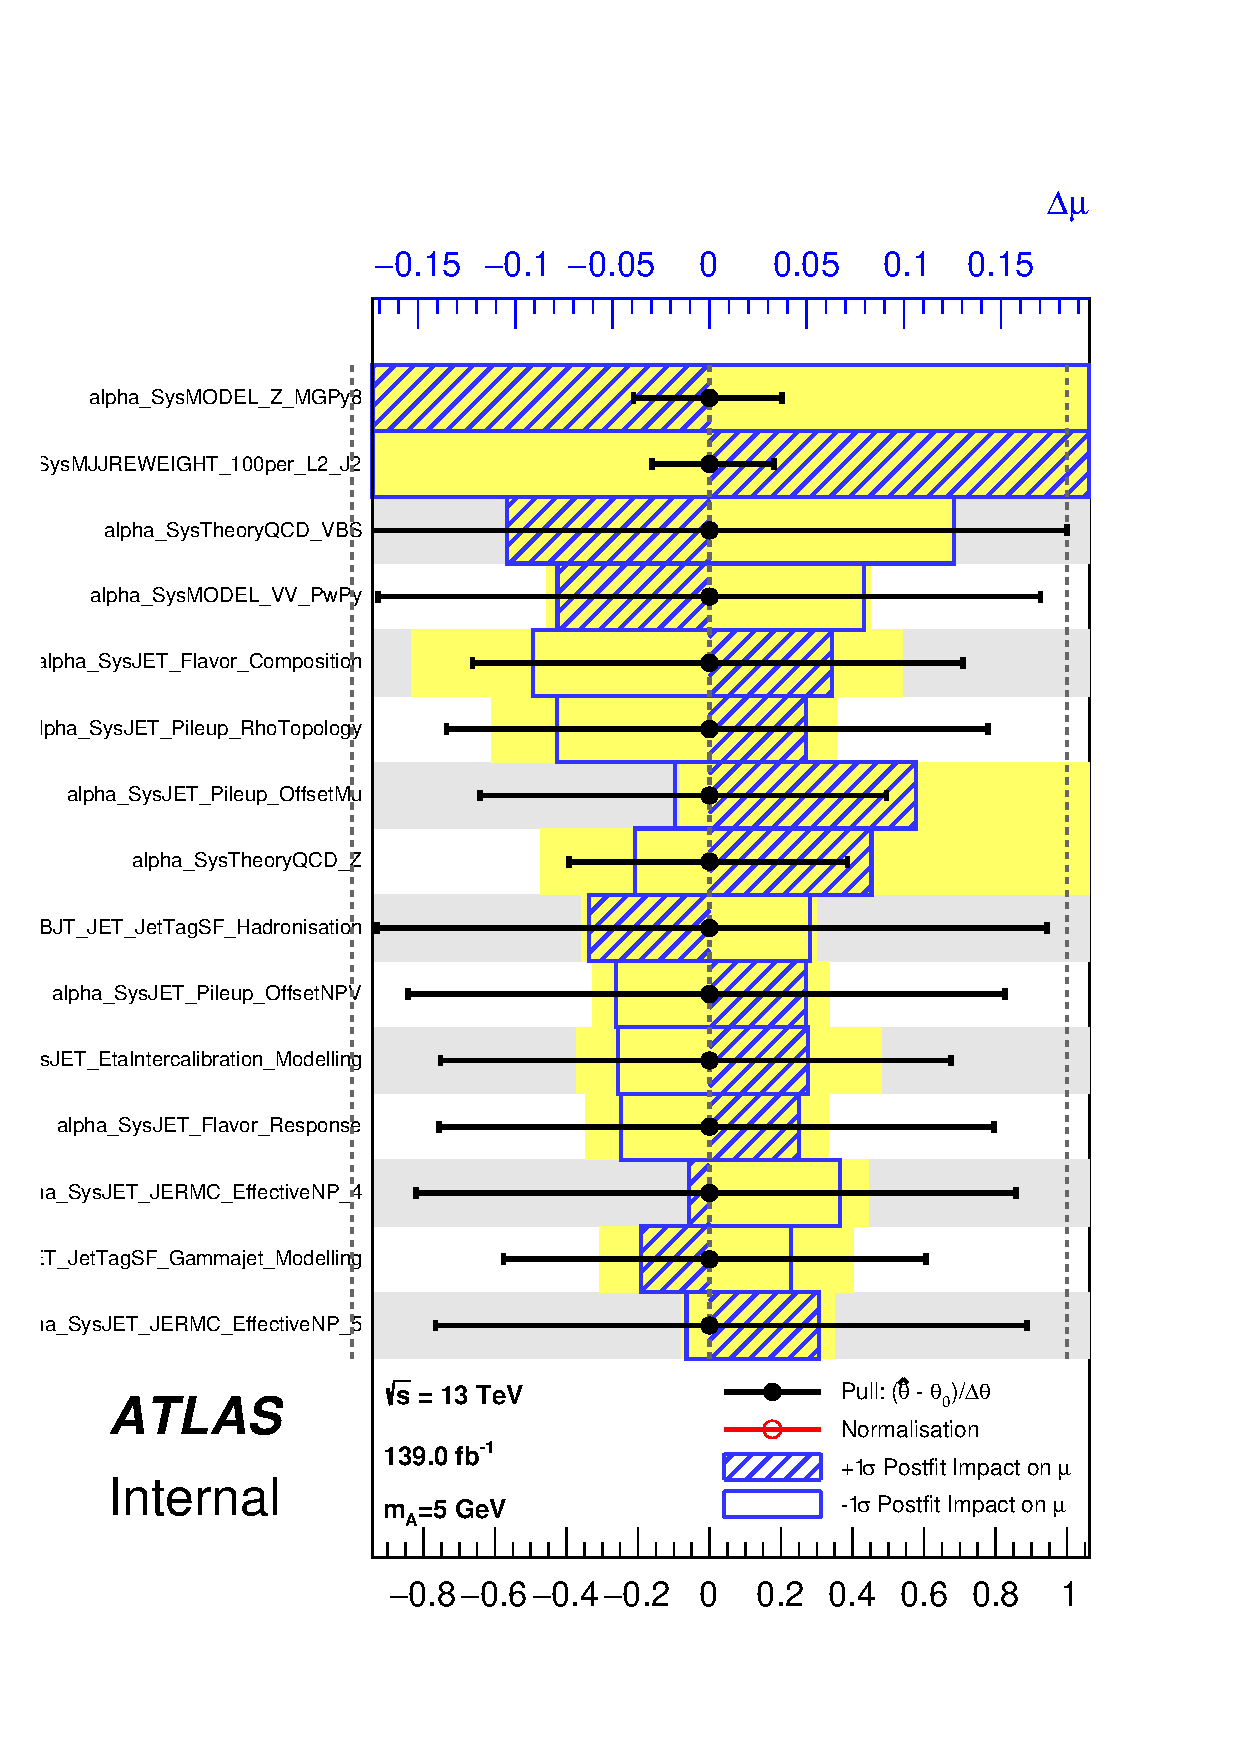
\includegraphics[width=0.8\textwidth]{figures/2lep/FitResults/pulls_mu_SemileptonicVBS_5_AsimovAllbins.pdf}
        \caption{Ranking plot for unconditional fit ($\mu=1$) to asimov data in the full range, for the 2 lepton channel only.}
       \label{fig:fit_2lep_ranking_all}
\end{figure}

\section{The observed signal strength}
The estimated signal strength in the fit is:
\begin{equation}
    %\mu = 0.982 \pm 0.217
    \mu = 0.98^{\plus 0.22}_{\minus 0.20} = 0.98^{\plus 0.09}_{\minus 0.09}(Stat)^{\plus 0.21}_{\minus 0.18}(Syst) 
\end{equation}
The corresponding observed (expected) significance is 5.90 (6.47)~$\sigma$, which shows the observation of the EW VV+jj signal in the semileptonic final state.

